%% main.tex
%% 主文档
\documentclass[11pt,a4paper,twoside,titlepage,hyperref,UTF8,fontset=mymac]{ctexbook}
%%%%<!-------------------- 增加功能 -------------------->
%% ctex设置
\ctexset{
    section/format = \Large\bfseries\raggedright,
    chapter = {
    	number = \arabic{chapter}
    },
    paragraph = {
    	beforeskip = 0pt
    },
	subsubsection = {
		numbering = true
	}
}
%% hyperref设置
\hypersetup{pdfborder=0 0 0}

%%%%<!-------------------- 增加功能 -------------------->
%% ams宏包
\usepackage{amsmath}
\usepackage{amssymb}
%% unicode-math宏包
\usepackage{unicode-math}
\setmainfont
[    Extension = .otf,
   UprightFont = *-regular,
      BoldFont = *-bold,
    ItalicFont = *-italic,
BoldItalicFont = *-bolditalic,
]{xits}
\setmathfont
[    Extension = .otf,
      BoldFont = *bold,
      bold-style = ISO
]{xits-math}
%% 图片宏包
\usepackage{graphicx}
%% 引用紧凑列表宏包
% \usepackage{mdwlist}

%% 化学式宏包
\usepackage[version=4]{mhchem}
%% textcomp宏包,显示单位
\usepackage{textcomp}
%% 分栏宏包
\usepackage{multicol}
%% 表格宏包
\usepackage{multirow}
%% 定义微分符号d
\newcommand{\diff}{\symrm{d }}
%% 定义常量pi
\newcommand{\cpi}{\symrm{\pi}}
%% 定义左对齐 右对齐
\newcommand{\alignleft}{\raggedright}
\newcommand{\alignright}{\raggedleft}

%%%%<!-------------------- 格式设置 -------------------->
%% 调整段落和页面格式
\usepackage[left=1.91cm, right=1.91cm, top=2.54cm, bottom=2.54cm]{geometry}
\setlength{\parskip}{0pt}
%% 调整目录
\usepackage{titlesec}
\usepackage{titletoc}
\titlecontents{chapter}[4em]{\vspace{3mm}\heiti}{\contentslabel{4.0em}}{}{\titlerule*[0.3pc]{.}\small\contentspage}
\titlecontents{section}[4em]{\normalsize}{\contentslabel{2.5em}}{}{\titlerule*[0.3pc]{.}\small\contentspage}
\titlecontents{subsection}[7em]{\normalsize\kaishu}{\contentslabel{3em}}{}{\titlerule*[0.3pc]{.}\small\contentspage}
%% 调整图标标题格式
\usepackage{caption}
\usepackage{subcaption}
\captionsetup{labelfont=bf,labelsep=quad}
%% 引用列表宏包调整列表格式
\usepackage[inline]{enumitem}
\setlist{topsep=0pt,partopsep=0pt,parsep=0pt,itemsep=0pt,itemjoin=\quad\quad}
%% 脚注每页重新标号
\usepackage[perpage]{footmisc}
%% 设置积分号
\usepackage[fourier]{varint}
%% 定制标题页、目录页和正文的格式
\newcommand{\docmaketitle}{\pagestyle{empty}\maketitle}
\newcommand{\doctableofcontents}{\frontmatter\pagestyle{headings}\tableofcontents\mainmatter}

%%%%<!-------------------- 文档设置 -------------------->
%% 包含文件
%\includeonly{Chapter03-机载LiDAR数据获取基本原理}

%% 文档属性
\title{\heiti{\Huge{激光遥感复习整理}}}
\author{\fangsong{\LARGE{胡奕公}}}
\date{}

%%%%<!-------------------- 正文 -------------------->
\begin{document}
%% 标题页
\pagestyle{empty}
\begin{titlepage}
	\centering
	\vspace{2cm}
	
\includegraphics[width=0.15\textwidth]{figure/透明底篮标}\par\vspace{0.5cm}
	{\scshape\LARGE 武汉大学遥感信息工程学院 \par}
	\vspace{2.5cm}
	{\scshape\Large\bfseries 激光遥感\par}
	\vspace{0.5cm}
	{\Huge\bfseries 复习整理\par}
	\vspace{2cm}
	{\Large\itshape 胡奕公\par}
	
	\vfill
	% Bottom of the page
	{\large \LaTeX \par}
\end{titlepage}

\doctableofcontents %% 目录
%% 正文开始
%% Chapter01-绪论.tex
%% 绪论
\chapter{绪论}

\section{基本概念}
\begin{itemize}
    \item \textbf{激光成像}:Laser Imaging, LI.
    \item \textbf{激光遥感}:Laser Remote Sensing, LRS.
    \item \textbf{激光雷达}:Light Detection And Ranging, LiDAR.
    \item \textbf{机载激光地形测绘}:Airborne Laser Terrain Mapping, ALTM.
    \item \textbf{机载激光制图}:Airborne Laser Mapping, ALM.
    \item \textbf{机载激光扫描}:Airborne Laser Scanning, ALS.
    \item \textbf{机载激光测高}:Airborne laser altimetry, ALA.
    \item \textbf{激光测高}:Laser Altimetry, LA.
    \item \textbf{机载激光扫描测高}:Airborne Laser Scanning Altimetry, ALSA.
    \item \textbf{空载光达、空载雷射扫描}:Light Detection And Ranging, LiDAR.
\end{itemize}

\section{应用现状}
\begin{enumerate}
	\item % 森林检测与管理
	\textbf{森林检测与管理}。LiDAR系统的最早商业应用领域之一。\\
	\textbf{传统技术}:以前是借助空中摄影和地面测量进行的。这些方法不仅费时费力,而且只能分析样点,结果还是推断的。\\
	\textbf{激光雷达的优势}:激光扫描法能克服这些缺点,通过激光扫描技术
	提取得完整的3D森林模型。在单个树木分析的基础上,可确定以下的参数:\begin{itemize}
		\item 单个树高
		\item 一片林区的平均树高
		\item 一片林区的木材体积
		\item 一片林区的平均密度
		\item 每片林区的平均生长体积
	\end{itemize} 
	此外LiDAR得到的DTM还可以来规划和改善森林运输道路,以及进行倾斜度分析,以便测定危险。
	\item % 构建数字城市模型
	\textbf{构建数字城市模型}:
	在电信、无线通讯、法律实施和灾难管理等众多领域中都需要准确的数字城市模型(建筑物建模、城市规划、噪声模拟、无线网络规划)
	\item % 湿地、限制进入地区、危险区域
	\textbf{湿地、限制进入地区、危险区域}
	\begin{itemize}
		\item 密集的植被覆盖和没有可通行的道路。
		\item 传统的地面摄像测量技术很难对沼泽、野生动物保护区及森林保护区进行勘测。
		\item 危险地带的地貌特征获取。
	\end{itemize}
	\item \textbf{油气管道勘测}
	\item \textbf{洪水灾情预测}(洪水制图、灾害评估)获取流域的数字表面模型和数字高程模型。
	\item \textbf{海岸线监测与制图}
	\item \textbf{水深、海岸线、侵蚀状况监测}
	\item \textbf{电力线监测}
	\item \textbf{股文物保护}
	\item \textbf{真正射影像的制作}
\end{enumerate}

\section{LiDAR技术特点}
\begin{enumerate}
	\item 无需光照条件或专门的太阳高度角。
	\item 可在白天、夜晚或相当恶劣的条件下(大雾)作业,全天时全天候获取地面三维数据。
	\item 能部分“穿透”植被,同时测量地面和非地面层。
	\item 很少需要进入测量现场,不需要大量的地面控制点。
	\item 能快速获取数据,24小时内可提取测区的DEM数据。
	\item 精度较高。
	\item 能够接受无穷次回波。
	\item 可在地面反射率比较低的区域工作,例如反射率只有约5\%的地面。
	\item 集成RS和GPS技术,数据可直接作为GIS的数据源,有利于提高地理数据的自动化,加快处理速度。
	\item 一个飞行日内可采集高达200 GB的数据。
	\item 高速度、高性能、高精度、长距离的航空测量设备。
	\item 全数字化,可直接产生三维坐标$ (X,Y,Z) $,无需其他额外步骤。
	\item 数据密集。基于固定翼机载平台采集时,典型的激光光斑中心间距为0.5 m左右。
	\item 精度:针对地物建模应用情形,典型精度达15 cm。
	\item 机载平台:便于操作,易于快速获取地表数据。
	\item 宽视场角:最大可以达到$ 75^{\circ} $的视场角。如果部分视场角范围没有被用到,可以用于飞机倾角稳
	定补偿。
\end{enumerate}

\section{激光成像技术}
\subsection{激光}
\paragraph{地位}\textit{激光}是20世纪以来,继原子能、计算机、半导体之后,人类的又一重大发明,被称为“最快的刀”、“最准的尺”、“最亮的光” 。
\paragraph{激光的亮度}约为太阳光的100亿倍。
\paragraph{激光的特点} \begin{itemize}
	\item 单色性、方向性、相干性
	\item 具有很高的单光子辐射能量
	\item 在大气传输中很少发生绕射
\end{itemize}
\paragraph{激光设备}1960年发明\textit{红宝石激光器},主要在军事上得到了应用。\begin{itemize}
	\item \textbf{激光测距仪}:美国1969年测地月距离。
	\item \textbf{激光致盲器}:1982年英阿马岛战争投入实战。
	\item \textbf{激光制导器}:1991年海湾战争,精度高、抗干扰能力强。
	\item \textbf{激光告警设备、激光干扰设备}等电子战装备。
\end{itemize}
\paragraph{激光的应用}\begin{itemize}
	\item \textbf{自然科学}
	\item \textbf{加工领域}
	\item \textbf{信息处理}
	\item \textbf{激光通信}
	\item \textbf{医学领域}
	\item \textbf{测绘领域}
	\item \textbf{环境检测}:弥补了微波在绕射和不能探测目标生化特性的不足,有了更加广泛的应用范围。 \begin{itemize}
		\item 大气成分探测(气溶胶探测)
		\item 污染探测大气和海洋基本参数,如:海水深度、温度等探测。
		\item 绿色植物探测
	\end{itemize}
\end{itemize}
\paragraph{微波雷达的局限性}\begin{itemize}
	\item 其波长较长,相应能量子的能量很小。
	\item 一般不足以与目标发生生化作用,无法探测目标的生化特性。
	\item 在传播过程中,遇到尺寸小于波长的物体时,更易于发生衍射。
\end{itemize}
\subsection{激光雷达与激光成像雷达}
\paragraph{激光雷达的光源类型}\begin{itemize}
	\item 可见光波段{\kaishu \ce{He}-\ce{Ne}和\ce{Ar}激光器}
	\item 短波红外波段{\kaishu Nd:YAG激光器}。最成熟的激光器。
	\item 长红外波段的{\kaishu \ce{CO2}激光器}。正在研制的大多是\ce{CO2}激光器,体积大,价格比较高。
	\item \textit{二极管泵浦固体激光雷达}(DPL),20世纪80年代后期。是发展重点。\\
	\textbf{DPL的优点}:\begin{itemize}
		\item 无需制冷
		\item 不像红外热成像系统容易受环境影响
		\item 对人眼安全,大气消光比低
		\item 可采用光纤光路和集成光学技术
		\item 结构小型化,体积小,制作成本低
		\item 具有高稳频、高功率、高效率和高光束质量等优点
		\item 可距离成像和强度成像
	\end{itemize}
	\textbf{DPL与其他激光器的比较}:\begin{itemize}
		\item \textbf{与Nd:YAG激光器相比}:后者只能测距和测角,不能测速,成像困难,大气传输性较差。
		\item \textbf{与\ce{CO2}激光器相比}:相干性好,寿命长,可靠性强。
	\end{itemize}
	\textbf{DPL的应用}\begin{itemize}
		\item 军事的应用
		\item 大气测污、风场测量、环境监测
	\end{itemize}
\end{itemize}
\paragraph{激光成像雷达的基本结构} 如图\ref{fig:激光成像雷达的基本结构}所示。
\begin{figure}[htbp]
	\centering
	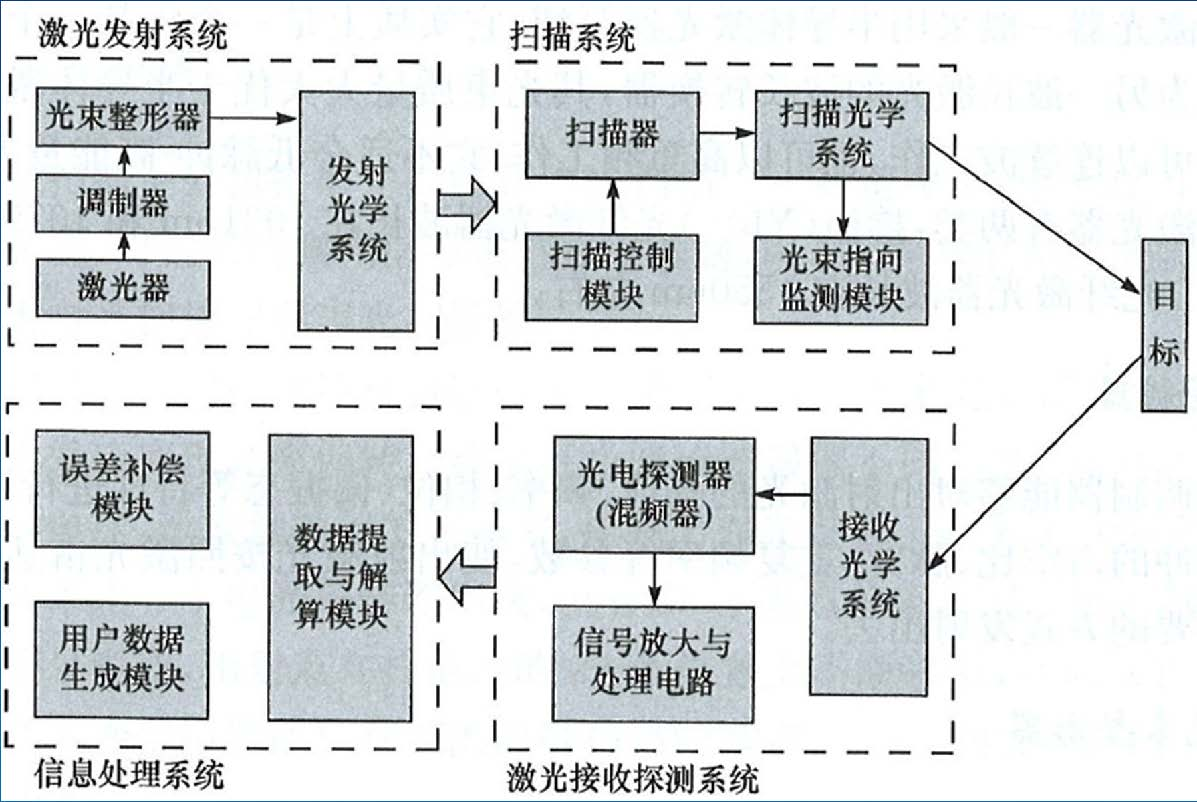
\includegraphics[width=0.7\linewidth]{figure/Chapter1/激光成像雷达的基本结构.jpg}
	\caption{激光成像雷达的基本结构}
	\label{fig:激光成像雷达的基本结构}
\end{figure}
\paragraph{激光成像雷达的发展}
\begin{itemize}
	\item 20世纪70年代,卫星激光测距(阿波罗登月计划)
	\item 1980至1988,机载LiDAR可行性研究。
	\item 1990年,斯图加特大学研制成功首个激光断面测 量系统
	\item 1993年,德国出现首个商用LiDAR系统TopScan(ALTM 1020)
	\item 1995年,全球有5套商用LiDAR系统
	\item 1999年,全球约有30几套商用LiDAR系统
	\item 2001年,全球约有75个公司使用了60几套商用LiDAR系统
	\item 2002年,全球约有120个公司使用了75几套商用LiDAR系统 ,年平均增长率为7.1\%,市场份额从5\%增长到12\%。
	\item 目前国内已引进20余套机载激光雷达系统。
\end{itemize}
\paragraph{激光雷达的新类型}\begin{enumerate}
	\item \textit{扫描激光雷达}\begin{itemize}
		\item 扫描成像激光雷达在对地观测领域最为成熟的应用是机载LiDAR系统。
		\item 采用单元探测器,每次测量只获得一个像素的数据,通过平台运动和扫描实现一定探测范围的成像。
		\item 机载LiDAR系统一般采用脉冲激光体制,要求激光的重复频率高,脉冲宽度窄,单脉冲能量大。
		\item 由记录的距离数据形成的图像称为距离图像,由记录的回波强度数据形成的图像称为强度图像。
	\end{itemize}
	\item \textit{凝视激光雷达(新型)}\\
	\textbf{原理}:凝视成像激光雷达需要控制发射激光,使发射光覆盖整个成像区域,然后通过面阵探测器接收回波,通过飞行时间测量或调制解调手段实现并行测距,得到目标三维图像。\\
	\textbf{优点}:凝视成像激光雷达实现了“瞬时”成像,具有结 构简单、成像速率高、像素分辨率高等诸多优点,有着广阔的应用前景。
	\item \textit{合成孔径激光雷达(新型)}\\
	\textbf{原理}:原理与微波合成孔径雷达类似,不同的是辐射源采用了激光波段。在距离向上发射大时宽带宽信号,对回波信号进行脉冲压缩得到距离向高分辨率;方位向上利用雷达平台与目标之间的相对运动,记录平台不同位置的目标回波信号,经相关的数据处理在空间上合成一个虚拟的大孔径,实现方位向聚焦,获得方位向的高分辨率。\\
	\textbf{优点}:合成孔径激光雷达是一种新型的主动式激光成像 雷达,它综合了传统的微波合成孔径雷达和激光雷达的优势。突破实孔径的衍射极限,当观测距离达到数百公里甚至更远时,它是唯一能够在有限的光学孔径条件下获得厘米级分辨率的光学成像手段。
\end{enumerate}

\subsection{激光雷达的关键技术}
下列四项技术中,前三项属于硬件技术,均已得到不同程度的解决;第四项技术属于软件技术,目前成为最关键的技术。
\begin{enumerate}
	\item \textit{激光发射器}:高功率和高波束质量的辐射源
	\begin{enumerate}
		\item \textit{气体激光器}\\	%% 气体激光器
		\textbf{特点}:\begin{itemize}
			\item 典型的气体激光器为\ce{CO2}
			\item 最早用于激光雷达的激光器之一
			\item 工作波长为10.6 \textmu m,处于大气窗口。
			\item 至今仍广泛用于激光雷达
		\end{itemize}
		\textbf{优点}:\begin{itemize}
			\item 大气传输性能好,效率高。
			\item \ce{CO2}激光雷达易于实现高灵敏度外差探测和三维成像,信息处理技术成熟。
		\end{itemize}
		\textbf{缺点}:\begin{itemize}
			\item 尺寸比较大
			\item 需要低温制冷
		\end{itemize}
		\item \textit{固体激光器}:应用非常广泛的Nd:YAG激光器 \begin{itemize}
			\item 在典型情况下,脉宽10~30 ns,单脉冲能量为100 mJ~1 J,脉冲重复率为10~100 Hz。
			\item 波长1.06 \textmu m的基频辐射YAG激光器可用于研究大气散射。
			\item 波长0.532 \textmu m的2倍频频光可用于海洋勘探。
			\item 波长0.355 \textmu m和0.266 \textmu m的3倍频和4倍频光可用于测污
		\end{itemize}
		\item \textit{半导体二极管激光器},又称半导体激光器又称激光二极管。\\ %% 半导体二极管激光器
		是用半导体材料作为工作物质的激光器。常用工作物质有砷化镓(\ce{GaAs})、硫化镉(\ce{CdS})、 磷化铟(\ce{InP})、硫化锌(\ce{ZnS})等。\\
		激励方式有电 注入、电子束激励和光泵浦三种形式。\\
		\textbf{特点}:半导体二极管激光器是最实用最重要的一类激光器。它体积小、寿命长,并可采用简单的注入电流的方式来泵浦其工作电压和电流与集成电路兼容,因而可与之单片集成。\\
	\end{enumerate}
	\item \textbf{成像探测器}:高灵敏度接收技术。\\ %% 成像探测器
	\textit{成像探测器}也称光电探测器(或混频器),是指将望远镜接收到的激光信号,直接转换成与之对应的电信号,或者将光信号与本振光混频,实现外差探测并将其转换成电信号。\\
	目前激光雷达采用的主流探测器包括:\textit{光电倍增管}(PMT)、\textit{雪崩光电二极管}(APD)、PIN\textit{光电二极管}、\textit{增强型电荷耦合器件}(ICCD)。\\
	激光雷达探测系统所采用的探测器一般有三种类型:\begin{enumerate}
		\item \textit{单元探测器}:\begin{itemize}
			\item 每次只获得一个像素的数据。
			\item 激光器每次发出宽度很窄的脉冲(一般以纳秒计)。
			\item 回波强度反映了目标的反射率特性。
			\item 使用扫描器控制发射脉冲按一定方式扫描,将光束指向不同目标,或目标上的不同位置。
			\item 通过接收系统形成图像,距离数据形成的图像称为距离图像,回波强度数据形成的图像称为强度图像。
			\item 要求激光重复频率高,脉冲宽度窄,单脉冲能量大。
			\item 激光成像雷达的高成像速率和高分辨率常常不能同时得到满足,采用单元探测器时,这一矛盾更加突出,所以需要折中考虑。
		\end{itemize}
		\item \textit{面阵探测器}:\begin{itemize}
			\item 需要控制发射激光,使发射光能覆盖较大面积的目标或同时照射许多不同的目标,然后接收回波信号。
			\item 需要对发射光进行调制,对接收信号进行解调,才能量测出距离。
			\item 不需要扫描器,但要求发射功率大。
			\item 无法采用高灵敏度的探测器。
			\item 在希望成像像素数多,成像速率要求不高的情况下采用。即在成像速率要求不高,成像分辨率要求很高的情况下采取的一种办法。
		\end{itemize}
		\item \textit{阵列探测器}:受限于器件技术以及信号处理技术水平,阵列探测器经历了单元模块阵列化、PIN阵列探测、APD阵列探测,及从线阵到面阵的发展阶段。\begin{itemize}
			\item \textbf{线阵探测}:需要将发射光分为$ N $束,同时照射目标上的$ N $点,从这些点上反射回来的信号由$ N $个探测元所接收,得到$ N $个像素上的距离信息和强度信息;
			\item 通过扫描器扫描,获得二维信息,对扫描器的要求比较高;
			\item 可以实现高速高分辨率成像。
			\item 技术难度较大
		\end{itemize}
	\end{enumerate}
	\item \textbf{扫描系统}:高性能二维扫描技术。用于激光成像雷达系统的扫描器目前可分为三种:力学、电学和二元光学扫描。
	\begin{enumerate}
		\item \textit{力学扫描器}:由反射镜转动或摆动使光束偏转进行大角度范围扫描。结构如图\ref{fig:力学扫描器结构}所示。
		\begin{figure}[htbp]
			\centering
			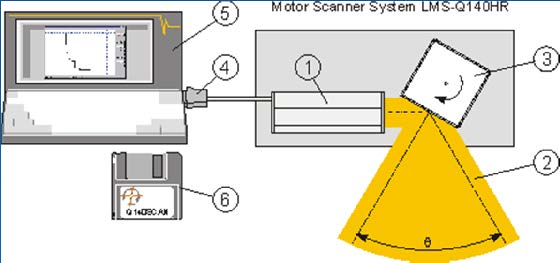
\includegraphics[width=0.7\linewidth]{figure/Chapter1/力学扫描器结构}
			\caption{力学扫描器结构}
			\label{fig:力学扫描器结构}
		\end{figure}\\
			\textbf{优点}:采用转镜可以达到很高的扫描速度,两个转镜可组成二维扫描系统。\\
			\textbf{缺点}:体积较大,笨重,耗电量大。
		\item \textit{声光电学扫描器}:\\
			\textbf{优点}:不包含机械运动,扫描速度快。\\
			\textbf{缺点}:\begin{itemize}
				\item 扫描角度小,一般为几十分之一毫弧度。
				\item 光透过率低,光束质量差。
				\item 耗电量大,光学系统必须作冷却处理。
			\end{itemize}
		\item \textit{二元光学扫描器}:利用二元光学技术制造,通过两组透镜的相对移动实现光束方向的偏转。\\
		\textbf{原理}:利用二元光学技术制造出来的微透镜阵列扫描器由间距只有几微米的微透镜阵列组成,分为两组:一组是正透镜,一组是负透镜。准直光经过透镜时会会聚光,然后通过负透镜时又变为准直光。正透镜阵列和负透镜阵列之间产生相对移动时,准直光的方向就会发生变化。两个微透镜阵列在水平方向相对移动时,输出光束在水平方向就会发生偏转。透镜之间微小的相对移动可以产生几度的光束偏转。\\
		\textbf{优点}:\begin{itemize}
			\item 扫描速度可以达到1KHz以上。
			\item 易于将一束光分为多束光。
			\item 扫描方式可通过编程任意加以改变。
			\item 体积小,重量小。
		\end{itemize}
		\textbf{缺点}:\begin{itemize}
			\item 但扫描角度较小,透过率较低。
			\item 尚未实用。
		\end{itemize}
	\end{enumerate}
	\item \textbf{数据处理技术}:图像处理及目标识别算法
\end{enumerate}

\section{激光遥感集成系统}
\paragraph{激光成像雷达的不足}虽然,激光成像雷达可以获取目标高精度的三维信息(包含高程信息和强度信息),但
\begin{itemize}
	\item 集成GPS/INS方可获取地标目标的绝对位置。
	\item 光谱、纹理信息缺乏,不利于地物识别。
\end{itemize}
\paragraph{激光遥感集成系统}随着数码相机等硬件技术的发展,将数码相机、GPS/INS与激光雷达集成,提高激光雷达的数据获取能力,已成为当前激光雷达系统获取数据的主要方式。(图\ref{fig:激光遥感集成系统})
\begin{figure}[htbp]
	\centering
	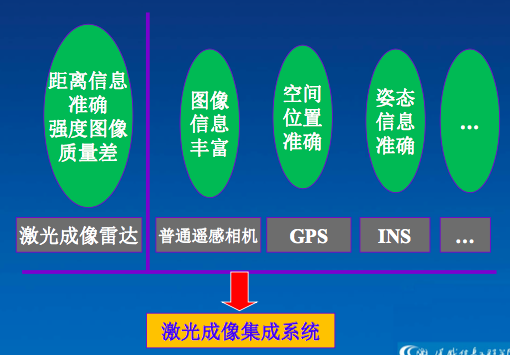
\includegraphics[width=0.7\linewidth]{figure/Chapter1/激光遥感集成系统}
	\caption{激光成像集成系统}
	\label{fig:激光遥感集成系统}
\end{figure}
\paragraph{激光遥感观测系统}由以下部分组成
\begin{itemize}
	\item 飞机
	\item 激光扫描仪
	\item 航摄相机
	\item 导航控制系统
	\item 高精度位置姿态测量系统(IMU/DGPS)
	\item IMU与相机连接架
	\item 机载DGPS天线
	\item 地面DGPS基站接收机
\end{itemize}
\paragraph{激光遥感集成系统的发展}\begin{enumerate}
	\item 美国航空航天局(NASA)最早支持开发激光成像三维测量的机载集成系统。
	\item 加拿大、瑞典、德国以及中国也相继开发出这类机载集成系统,可用于陆地和浅海水下地形测量。
\end{enumerate}
\section{国内常见LiDAR系统的扫描方式}
\paragraph{摆镜扫描}Leica、Optech采用的扫描方式。如图\ref{fig:摆镜扫描方式}所示。
\begin{figure}[htbp]
	\centering
	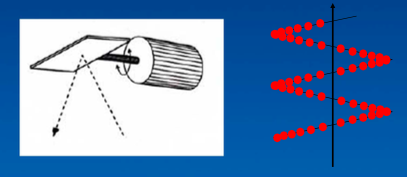
\includegraphics[width=0.7\linewidth]{figure/Chapter1/摆镜扫描方式}
	\caption{摆镜扫描方式图示}
	\label{fig:摆镜扫描方式}
\end{figure}
\paragraph{旋转棱镜扫描}Toposys Harrier、Riegl、IGS采用。如图\ref{fig:旋转棱镜扫描方式}所示。
\begin{figure}[htbp]
	\centering
	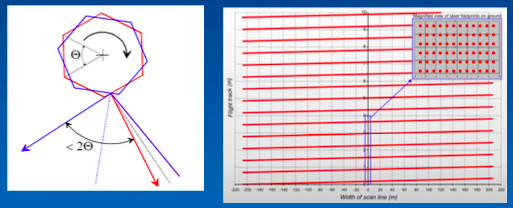
\includegraphics[width=0.7\linewidth]{figure/Chapter1/旋转棱镜扫描方式}
	\caption{旋转棱镜扫描方式}
	\label{fig:旋转棱镜扫描方式}
\end{figure}
\paragraph{光线扫描方式}Toposys Falcon系列。如图\ref{fig:光纤扫描方式}所示。
\begin{figure}[htbp]
	\centering
	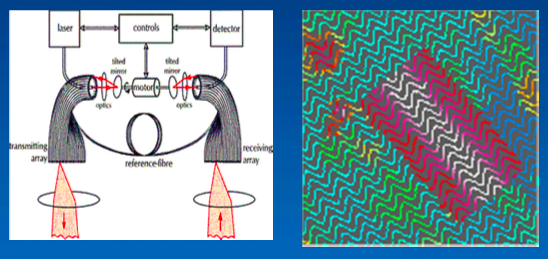
\includegraphics[width=0.7\linewidth]{figure/Chapter1/光纤扫描方式}
	\caption{光纤扫描方式}
	\label{fig:光纤扫描方式}
\end{figure}
\paragraph{圆锥镜扫描方式}opEye MK 系列、国产三维激光成像仪采用。如图\ref{fig:圆锥镜扫描方式}所示。
\begin{figure}[htbp]
	\centering
	\subfloat[圆锥镜扫描原理]{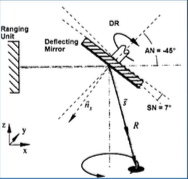
\includegraphics[height=4cm]{figure/Chapter1/圆锥镜扫描_原理}}
	\subfloat[圆锥镜扫描脚点形状]{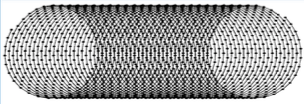
\includegraphics[height=4cm]{figure/Chapter1/圆锥镜扫描_脚点}}
	\caption{圆锥镜扫描方式}。
	\label{fig:圆锥镜扫描方式}
\end{figure}
\section{机载激光三维测量系统对比}
如图\ref{fig:机载激光三维测量系统对比}。
\begin{figure}[!htbp]
	\centering
	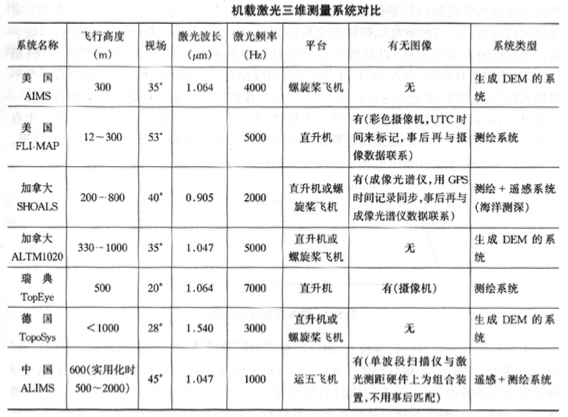
\includegraphics[width=1\linewidth]{figure/Chapter1/机载激光三维测量系统对比}
	\caption{机载激光三维测量系统对比}
	\label{fig:机载激光三维测量系统对比}
\end{figure}

% !TeX root = main.tex
%% Chapter02-激光及激光雷达系统.tex
%% 激光及激光雷达系统
\chapter{激光及激光雷达系统}

\section{激光} %% Section 1 	激光
\textit{激光}(Light Amplification by Stimulated Emission of Radiation, Laser),即“光的手机辐射放大”。

\subsection{辐射与原子} %% Subsection 1.1	辐射与原子
\paragraph{辐射与原子的相互作用的三种过程} \begin{enumerate}
	\item 
		\textit{自发辐射跃迁}:较高能级的粒子,自发地发射一个光子,跃迁到较低能级。其过程如图\ref{fig:自发辐射跃迁}所示。
		\begin{figure}[htbp]
			\centering
			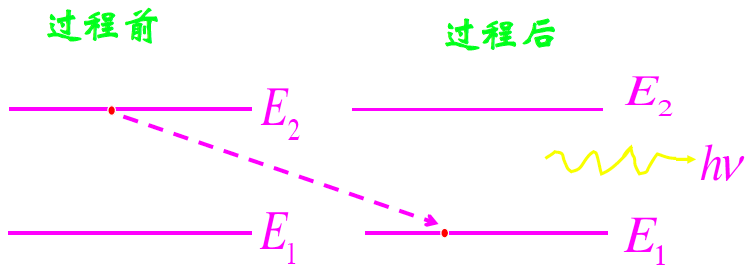
\includegraphics[width=0.7\linewidth]{figure/Chapter2/自发辐射跃迁}
			\caption{自发辐射跃迁}
			\label{fig:自发辐射跃迁}
		\end{figure}
		
		\textbf{光子的频率}为\begin{equation} \nu = \dfrac{E_2-E_1}{h} \end{equation}其中,$ h $是普朗克常量,$ h=6.624 \times 10^{-34} \ \symrm{\mu m} $。
		
		\textbf{自发辐射的速率}为\begin{equation} A_{21} = \dfrac{\diff n_{21}}{\diff t} \dfrac{1}{n_2} \end{equation}
		自发辐射速率的倒数表示由自发辐射所决定的有限寿命\begin{equation} \tau = \dfrac{1}{A_{21}} \end{equation}
		
		具有两个能级的原子系统在外来辐射的作用下可能产生两种过程:\begin{itemize}
			\item 处于低能级E1的原子在外来辐射作用下,吸收一个光子后向高能级E2跃迁(受激吸收过程);
			\item 处于高能级E2的原子在外来辐射作用下,发射一个与入射光子属于同一光子态的光子,并向低能E1级跃迁(受激辐射过程);
		\end{itemize} % 具有两个能级的原子系统在外来辐射的作用下可能产生两种过程
	\item 
		\textit{受激吸收跃迁}:较低能级的粒子吸收一个光子,跃迁到较高能级。其过程如图\ref{fig:受激吸收跃迁}所示。
		\begin{figure}[htbp]
			\centering
			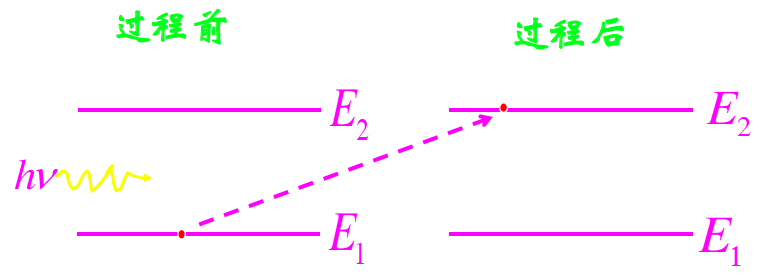
\includegraphics[width=0.7\linewidth]{figure/Chapter2/受激吸收跃迁}
			\caption{受激吸收跃迁}
			\label{fig:受激吸收跃迁}
		\end{figure}
	\item 
		\textit{受激辐射跃迁}:较高能级的粒子在光子激励下跃到较低能级,并发射一个同频率光子。其过程如图\ref{fig:受激辐射跃迁}所示。
		\begin{figure}[htbp]
			\centering
			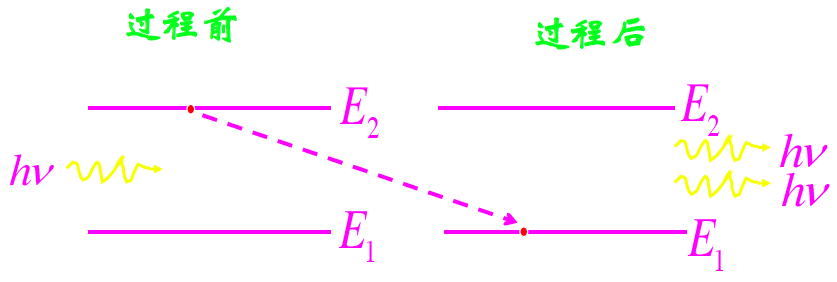
\includegraphics[width=0.7\linewidth]{figure/Chapter2/受激辐射跃迁}
			\caption{受激辐射跃迁}
			\label{fig:受激辐射跃迁}
		\end{figure}
\end{enumerate} % 辐射与原子的相互作用的三种过程

\subsection{受激辐射放大} %% Subsection 1.2	受激辐射放大
\paragraph{外来辐射场的作用}原子系统会产生受激吸收过程和受激辐射过程。\begin{itemize}
	\item \textit{受激吸收过程}:具有一定频率的光子消失的过程,表现为能量由外来辐射场向原子转移,导致辐射场的衰减。
	\item \textit{受激辐射过程}:是原子系统不断产生具有一定频率的光子,表现为能量由原子向辐射场的转移,使辐射场增强。
\end{itemize} % 外来辐射场的作用
一般说来,这两种过程总是同时存在。\begin{itemize}
	\item 如果受激吸收过程占主导地位,最终结果则是辐射场衰减;
	\item 而如果受激辐射过程起主导作用,最终结果就是辐射场的增强。
\end{itemize}% 两种作用同时存在

\paragraph{辐射场增强的条件}在某一段时间$ \diff t $内,由于受激辐射而从能级$ E_1 $向能级$ E_2 $跃迁的原子数为
\begin{equation} \diff n_{12}=n_1W \diff t \end{equation}
由于受激辐射作用而从从能级$ E_2 $向能级$ E_1 $跃迁的原子数为\begin{equation} \diff n_{21}=n_2W \diff t \end{equation}这里假定$ W_{12} = W_{21} = W $。

在两种过程共同作用下,光子的净增量可以表示为
\begin{equation} \Delta N = \left(n_2W - n_1W\right)\diff t = \delta nW\diff t \end{equation}
其中$ \Delta n = n_2-n_1 $。

\textbf{入射光经过原子系统后得到增强的条件}:处于能级E2上的粒子数多于能级E1上粒子数。

根据玻尔兹曼分布定律,处于热平衡状态时,有
\begin{equation} \dfrac{n_2}{n_1} = e^{\frac{E_2-E_1}{kT}} < 1 \end{equation}
即,辐射光通过处于热平衡状态的原子系统时,是辐射场的衰减。

\textbf{粒子反转分布状态}:要使得辐射场得到增强,必须使原子系统的分布为$ n_2>n_1 $。
以某种方式向原子系统提供能量,将足够多的粒子从能级$ E_1 $抽运到$ E_2 $。

\subsection{激光的产生} %% Subsection 1.3	激光的产生
\paragraph{工作物质}原子系统在获得能量后,处于粒子数反转分布状态,称之为\textit{激光工作物质}。工作物质的特点:\begin{itemize}
	\item 工作物质自身某些原子的自发辐射产生的光子, 在传播过程中会作为入射光引起其它原子受激跃迁。
	\item 工作物质处于粒子数反转分布状态,若受激辐射跃迁超过受激吸收跃迁,则光在传播中会得到激励和放大。
	\item 只要工作物质足够长,即使初始信号很小,也会被放大得很强。
\end{itemize}

\paragraph{激光产生的条件}\begin{itemize}
	\item 工作物质处于粒子数反转分布状态。
	\item 受激辐射跃迁超过受激吸收跃迁。
	\item 传播中的光得到激励和放大。
\end{itemize}

\paragraph{激光产生的过程}在工作物质两端分别放置一块反射镜,构成一个\textit{光学谐振腔}。工作物质由抽运系统被抽运到粒子数反转分布状态,因自发辐射而产生的向各个方向传播的光子,在光学谐振腔的作用下,沿着腔轴方向传播的光就会因两端的反射镜往返传播,并很快得到放大。那些传播方向与腔轴方向有一定夹角的光在几次往返后会逸出腔外。由于受激辐射占主导地位,沿腔轴往返传播的光由于受激辐射迅速放大,形成\textit{自激振荡},产生了激光。

受激辐射场与激励场具有相同的频率、相位、传播方向和偏振态,即\textbf{受激辐射光子和激励光子属于同一光子态},所以激光束具有很好的方向性、单色性、相干性。

\begin{figure}[!htbp]
	\centering
	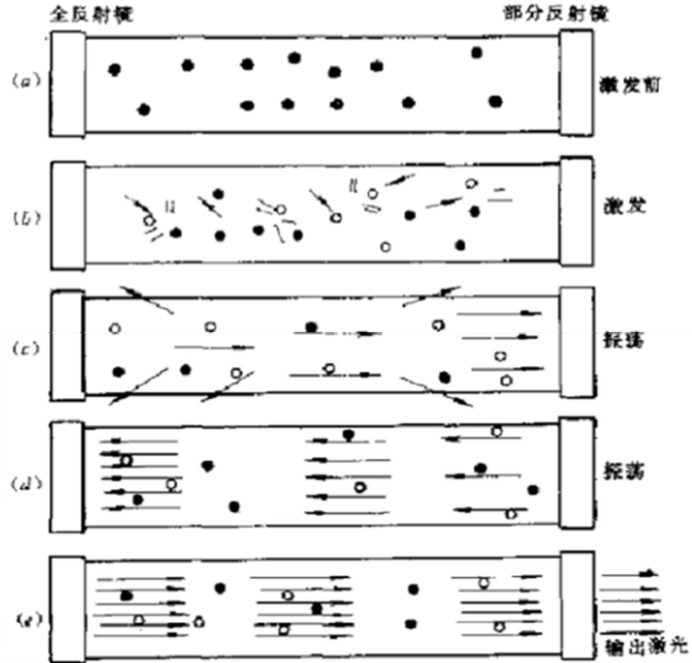
\includegraphics[width=0.6\linewidth]{figure/Chapter2/激光的产生过程}
	\caption{激光产生过程}
	\label{fig:Chpater2-激光产生过程}
\end{figure}

\section{激光器} %% Section 2	激光器

\paragraph{激光器}产生激光的装置称为激光器,激光器虽然多种多样,但其目的都是通过激励和受激辐射放大而获得激光。
\paragraph{激光器的组成}\begin{itemize}
	\item 工作物质
	\item 抽运系统
	\item 光学谐振腔
\end{itemize}
\paragraph{激光器的分类}
\begin{multicols}{2}
	\begin{itemize}
		\item \textbf{按照工作物质分类} 
			\begin{itemize}
				\item 固体激光器
				\item 气体激光器
				\item 液体激光器
				\item 半导体激光器
				\item 自由电子激光器
			\end{itemize} % 按照工作物质分类
		\item \textbf{按转运方式分类}
			\begin{itemize}
				\item 连续激光器
				\item 单次脉冲激光器
				\item 重复脉冲激光器
				\item 锁模激光器
				\item 单模和稳频激光器
				\item 可调谐激光器
			\end{itemize} % 按转运方式分类
		\item \textbf{按激励方式分类}
			\begin{itemize}
				\item 光泵式激光器
				\item 电激励式激光器
				\item 化学激光器
				\item 核泵浦激光器
			\end{itemize} % 按激励方式分类
		\item \textbf{按照输出波段范围分类}
			\begin{itemize}
				\item 远红外激光器
				\item 中红外激光器
				\item 近红外激光器
				\item 可见激光器
				\item 近紫外激光器
				\item 真空紫外激光器
				\item X射线激光器
			\end{itemize} % 按照输出波段范围分类
	\end{itemize}
\end{multicols}

\paragraph{激光的应用}\begin{itemize}
	\item \textbf{自然科学}
	\item \textbf{加工领域}
	\item \textbf{信息处理}
	\item \textbf{激光通信}
	\item \textbf{医学领域}
	\item \textbf{军事领域}
\end{itemize}

\paragraph{未来激光器的发展}
\begin{itemize}
	\item 实用角度
	\item 波长角度
	\item 输出功率
	\item 新类型激光器
\end{itemize}

\subsection{气体激光器} %% Subsection 2.1	气体激光器
\paragraph{用于激光雷达的气体激光器}主要有:\begin{itemize}
	\item \ce{CO2}激光器
	\item \ce{BrHg}激光器
	\item \ce{N2}分子激光器
	\item 准分子激光器
\end{itemize}

工作波长从近紫外到红外;以强放电激励为基本能源。

\paragraph{\ce{CO2}激光器}\ce{CO2}激光器是最早用于激光雷达的激光器之一,工作波长工作波长为10.6 μm,处于大气窗口。至今仍广泛用于激光雷达。

\paragraph{\ce{CO2}分子的震动方式}\ce{CO2}分子的3个原子呈对称排列,震动方式如图\ref{fig:CO2分子的震动方式}所示。
\begin{figure}[htbp]
	\centering
	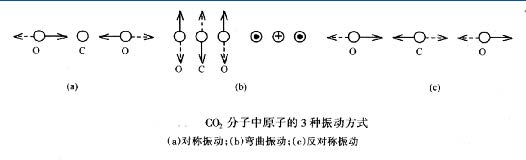
\includegraphics[width=\linewidth]{figure/Chapter2/CO2分子的震动方式}
	\caption{\ce{CO2}分子的震动方式}
	\label{fig:CO2分子的震动方式}
\end{figure}

\paragraph{\ce{CO2}激光器的优点}\begin{itemize}
	\item \ce{CO2}激光器工作波长工作波长为10.6 μm,对人眼安全。
	\item 具有优良的大气传输性能。
	\item 有较大的输出功率和能量转换效率。
	\item 易于进行外差探测。
\end{itemize}

\paragraph{\ce{CO2}激光器的缺点}\begin{itemize}
	\item 需要低温制冷。
	\item 目标对10.6 μm的激光反射率低,且\ce{CO2}激光易被水分子吸收。
\end{itemize}

\paragraph{\ce{CO2}激光器的跃迁机理}
\begin{enumerate}
	\item 
		\textbf{由分子在基态电子能级的振动子能级间跃迁产生}。在放电激励情况下,两种跃迁方式:
		\begin{itemize}
			\item 基态电子能级中(000)振动子能级上的分子与激励电子碰撞,被直接激发到激光能级(001)上,即:
				\begin{equation} \ce{CO2(000) + e\text{(高能)} -> CO2(001) + e\text{(低能)} } \end{equation}
			\item 具有较高的振动子能级分子与其它处于(000)能级上的分子发生碰撞, 跃迁到激光能级(001)。
		\end{itemize}
		两种可能的跃迁方式概率都不大。
	\item 
		\textbf{为了提高跃迁概率,在\ce{CO2}中掺入少量的\ce{N2}气体}。基态电子能级中V=0的振动子能级上的N2分子,被激励电子碰撞后跃迁到V=1的振动能级与CO2的(001)能级接近,很容易将能量转移到处于(000)能级的CO2分子,使它跃迁到(001)能级。即
		\begin{equation} \ce{ CO2(000) + N2(V=1) -> CO2(001) + N2(V=0) } \end{equation}\\
		\textbf{优点}:\ce{N2}分子基态电子能级的V=1子能级寿命相当长,可以积累大量\ce{N2}分子,使较多\ce{CO2}分子从(000)能级跃迁到(001)能级。\\
		\textbf{增加输出功率}:\begin{itemize}
			\item 进一步加入氦气可以使激光输出功率几倍地增大。
			\item 加进适量氙气(\ce{Xe}),也能使其增加输出功率。
			\item 加入适量的水蒸汽(\ce{H2O}),可使激光输出功率显著地增加。
		\end{itemize}
		\textbf{延长激光器的寿命}:在\ce{CO2}激光器里加入氢气(\ce{H2})、一氧化碳(\ce{CO})和氧气(\ce{O2})将延长激光器的寿命。
\end{enumerate}

\subsection{固体激光器} %% Subsection 2.2	固体激光器

\paragraph{常见的固体激光器} Nd:YAG激光器、钛宝石激光器等。

\paragraph{固体激光器的特点}\begin{itemize}
	\item 一般体积较小,与气体激光器相比更加可靠。
	\item 应用十分广泛。
\end{itemize}

\paragraph{Nd:YAG激光器} \begin{itemize}
	\item \textbf{化学组成}:是以钇铝石榴石晶体(化学式是\ce{Y3Al5O15},简称为YAG)为基质,掺入约1\%的激活离子\ce{Nd^3+}就成为Nd:YAG。
	\item \textbf{应用}:用于遥感的Nd:YAG激光器,在典型情况下脉宽10$ \sim $30 ns,单脉冲能量为100 mJ$ \sim $1 J,脉冲重复率为10$ \sim $100 Hz。
		\begin{itemize}
			\item 波长1.06 μm的基频辐射YAG激光器可用于研究大气散射。
			\item 波长0.532 μm的2倍频频光可用于海洋勘探。
			\item 波长0.355 μm和0.266 μm的3倍频和4倍频光可用于测污。
		\end{itemize}
\end{itemize}

\paragraph{二极管泵浦YAG激光器}由于固体激光器在相干性、脉冲重频和输出功率等方面受到局限,遇到CO2 激光器的挑战。寻求新的泵浦方法即二极管泵浦YAG激光器。
\begin{itemize}
	\item \textbf{优点}:泵浦效率高,输出功率高,寿命长。
	\item \textbf{缺点}:结构复杂,成本较高。
\end{itemize}
二极管泵浦Nd:YAG激光器的结构,如图\ref{fig:激光二极管泵浦YAG激光器}所示。
\begin{figure}[htbp]
	\centering
	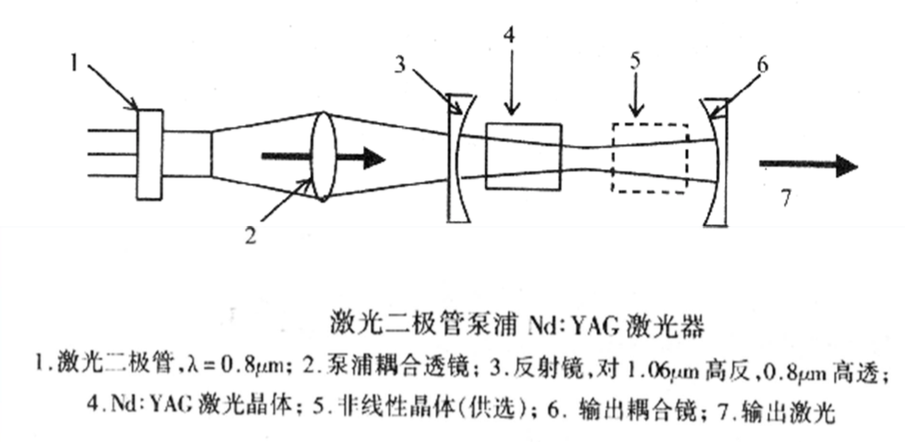
\includegraphics[width=0.7\linewidth]{figure/Chapter2/激光二极管泵浦YAG激光器}
	\caption{二极管泵浦Nd:YAG激光器的结构}
	\label{fig:激光二极管泵浦YAG激光器}
\end{figure}

\paragraph{固体可调谐激光器} 
\begin{itemize}
	\item \textbf{作用}:激光雷达探测对象的响应特性与激光波长密切相关,波长可调的激光器十分有用。
	\item \textbf{类型}:
		\begin{itemize}
			\item 1979年Walling等发明\textit{翠绿宝石激光器}
				\begin{itemize}
					\item 早期有较高实用价值的固体可调谐激光器。
					\item 波长调谐范围是700 $ \sim $ 830 nm。
				\end{itemize} % 翠绿宝石激光器
			\item 1982年Moulton发明\textit{钛宝石激光器}
				\begin{itemize}
					\item 一个重要的进展。
					\item 钛宝石激光晶体的基质是\ce{Al2O3},其中少量的\ce{Al^3+}被\ce{Ti^3+}取代(便于产生激光)。
					\item 钛宝石在400$ \sim $600 nm范围内具有很宽的吸收带,发射带为660$ \sim $1160 nm,波长调谐范围很宽。
					\item 虽然钛宝石具有较大的受激发射截面,增益较高,但激光能级的寿命只有3.2 μs,通常用其它激光器作抽运工作:氩离子激光器、铜蒸气激光器、2倍频Nd:YAG激光器。
				\end{itemize}
		\end{itemize} % 类型
\end{itemize} % 固体可调谐激光器

\subsection{半导体二极管激光器} %% Subsection 2.3	半导体二极管激光器
\paragraph{半导体二极管激光器的特点}
\begin{itemize}
	\item 完全不同的物理机制。
	\item 半导体材料中的电子智能存在于两个能带之一,每个能带所包含的能级数等于晶体中的原子数。根据Pauli不相容原理,每个能级上只能有一个电子。
	\item 半导体材料多是晶体结构。当大量原子规则而紧密地结合成晶体时,晶体中那些价电子都处在晶体能带\footnote{价电子所处的能带称\textit{价带}(对应较低能量)。与价带最近的高能带称\textit{导带},能带之间的空域称为\textit{禁带}}上。本征半导体的能带结构如图\ref{fig:本征半导体能带结构}所示。
		\begin{figure}[htbp]
			\centering
			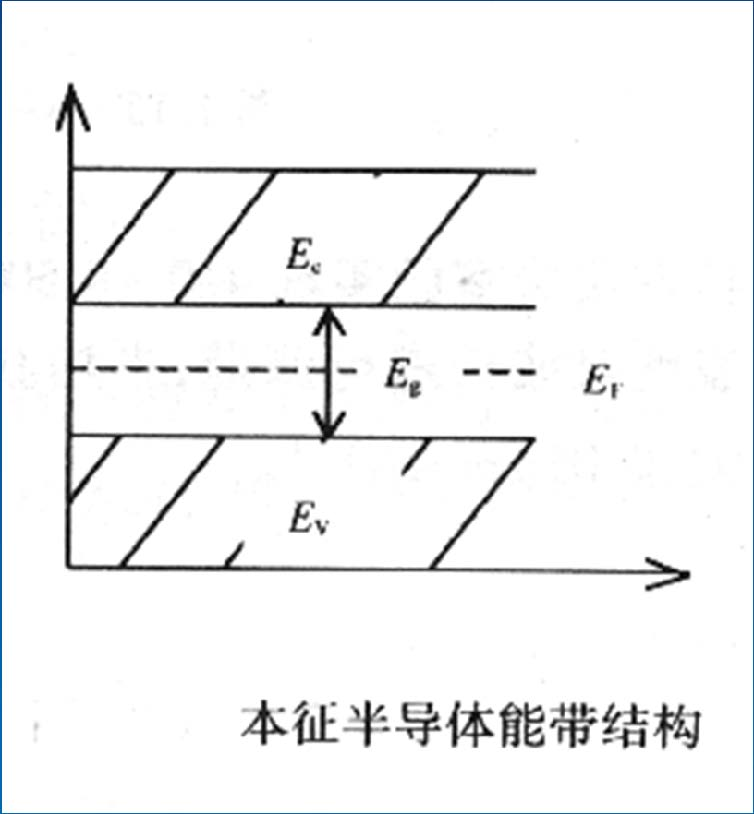
\includegraphics[width=0.3\linewidth]{figure/Chapter2/本征半导体能带结构}
			\caption{本征半导体能带结构}
			\label{fig:本征半导体能带结构}
		\end{figure}
	\item 电子不能再两个能带之间(禁带)驻留。
	\item 没有杂质的纯净半导体,称为本征半导体。
\end{itemize}

\paragraph{半导体二极管激光器的工作原理}
\begin{enumerate}
	\item 如果在本征半导体中掺入杂质原子,则在导带之下和价带之上形成了杂质能级,分别称为施主能级和受主能级。
		有施主能级的半导体称为\textit{n-型半导体};有受主能级的半导体称为\textit{p-型半导体}。
	\item 由于p-半导体与n-半导体所处能级不一致,高低能级的载流子作扩散运动,最终形成\textit{p-n结},此时处于热平衡状态,具有统一的Fermi能级。该过程如图\ref{fig:p-n结}所示。
		\begin{figure}[htbp]
			\centering
			\includegraphics[width=0.5\linewidth]{figure/Chapter2/P-N结}
			\caption{p-n结}
			\label{fig:p-n结}
		\end{figure}
	\item 若加偏压,在结区形成窄区域,导带(高能级)底部能级被电子占据, 价带(低能级)顶部被空穴占据;当导带电子回到价带, 与空穴发生受激复合时就产生了激光。该过程如图\ref{fig:p-n结产生激光}所示。
		\begin{figure}[htbp]
			\centering
			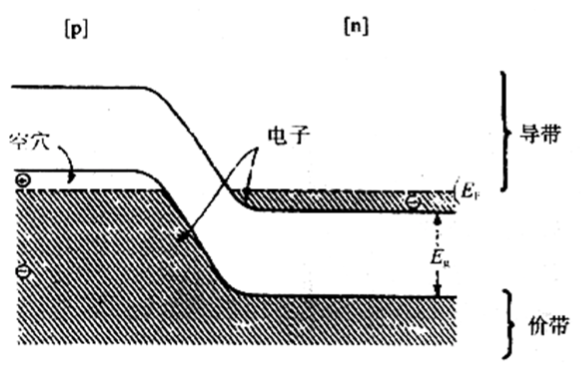
\includegraphics[width=0.5\linewidth]{figure/Chapter2/p-n结产生激光}
			\caption{p-n结产生激光}
			\label{fig:p-n结产生激光}
		\end{figure}
\end{enumerate}

\section{激光雷达系统} % Section 3	激光雷达系统
\subsection{激光雷达系统概述} % SubSection 3.1	激光雷达系统概述

\paragraph{激光雷达的产生}雷达工程师努力探索更短波长的辐射源,在微波振荡器的基础上,发明了激光器,将其与雷达技术相结合,产生了激光雷达技术。

\paragraph{激光雷达的特点}
\begin{itemize}
	\item 角分辨率较高
	\item 距离和速度分辨率高
	\item 抗干扰能力强
	\item 能够与一些目标发生生化作用
	\item 可以对极小的目标进行探测激
\end{itemize}

\paragraph{激光雷达的要求} 激光雷达要求具备发射高功率、窄脉宽、窄频带、较小远场发散角光束较高的脉冲频率的激光器。

\paragraph{激光雷达系统的分类}
\begin{enumerate}
	\item \textbf{按照使用目的分类}
		\begin{itemize}
			\item 探测环境状态
				\begin{itemize}
					\item \textbf{大气}:气溶胶分布、云、气象因素、污染物质……
					\item \textbf{水体}:浮游生物、水温、海洋污染……
					\item \textbf{陆地}:植物生长、热岛效应、污染状况……
				\end{itemize} % 探测环境状态
			\item 量测距离
				\begin{itemize}
					\item \textbf{太空}:星球间距离、星球地形……
					\item \textbf{海洋}:水体深度、水下地形……
					\item \textbf{陆地}:地形图、数字高程模型、植被提取……
				\end{itemize} % 量测距离
		\end{itemize} % 按照使用目的分类
	\item \textbf{按激光和物质的相互作用分类}
		\begin{itemize}
			\item \textbf{反射}:检测比激光波长大很多的物体。地形测绘。
			\item \textbf{米氏散射}:检测微粒直径与激光波长相等的物质。气溶胶。
			\item \textbf{瑞利散射}:检测微粒直径与激光波长小很多的物质。空气分子。
			\item \textbf{拉曼散射}:具有震动和旋转能力的分子。空气分子、水蒸气、\ce{SO2}等污染物质。
			\item \textbf{荧光法}:具有共振能级的分子和原子。\ce{NO2}等污染物质。
		\end{itemize} % 按激光和物质的相互作用分类
	\item \textbf{按使用的激光器分类}
	\item \textbf{按脉冲方式或连续波方式分类}
	\item \textbf{按光波检测的方法分类}
	\item \textbf{按工作台分类}
	\item \textbf{按接收的信号\footnote{激光雷达接收的信号:\begin{itemize}
			\item 可能是反射信号
			\item 也可能是大气散射信号(被称为弹性散射)
			\item 吸收衰减信号、共振散射信号、荧光信号等
	\end{itemize}}分类}
		\begin{itemize}
			\item \textit{反射型激光雷达系统}:地形测绘。
			\item \textit{散射型激光雷达系统}:探测大气中低浓度的尘埃
			\item \textit{吸收性激光雷达系统}:估计某种成分的平均密度
			\item \textit{激光荧光系统}:探测大气中的微量元素
		\end{itemize}
\end{enumerate} % 激光雷达系统的分类

\paragraph{双视场米氏散射激光雷达}武汉大学研制的双视场米氏散射激光雷达,主要由激光发射系统、光学接收系统和信号检测系统组成。

\paragraph{激光雷达系统的结构} 
\begin{itemize}
	\item \textit{双稳系统}:发射部分和接收部分分开放置,目的是为了提高空间分辨率。由于目前脉宽为ns级的激光已达到很高空间分辨率,因此该系统已经很少被采用。双稳系统结构框图如图所示。
		\begin{figure}[htbp]
			\centering
			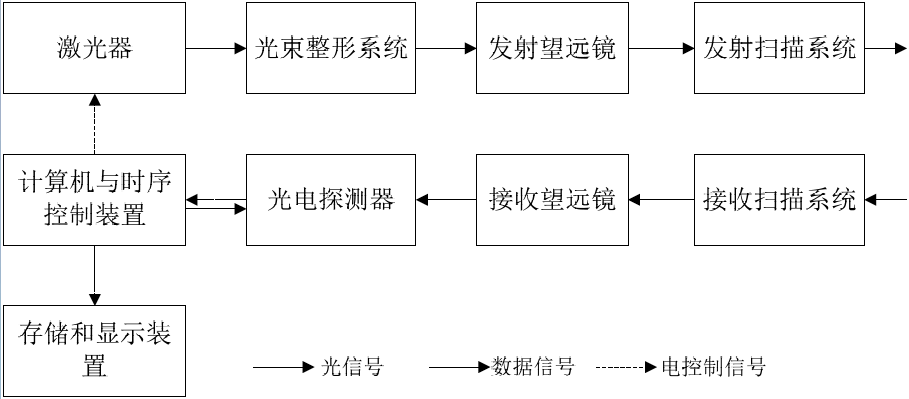
\includegraphics[width=0.7\linewidth]{figure/Chapter2/双稳系统的结构框图}
			\caption{双稳系统的结构框图}
			\label{fig:双稳系统的结构框图}
		\end{figure}
	\item \textit{单稳系统}:发射与接收信号共用一光学子系统,由发送/接收(T/R)开关隔开。单稳系统结构框图如图所示。
		\begin{figure}[htbp]
			\centering
			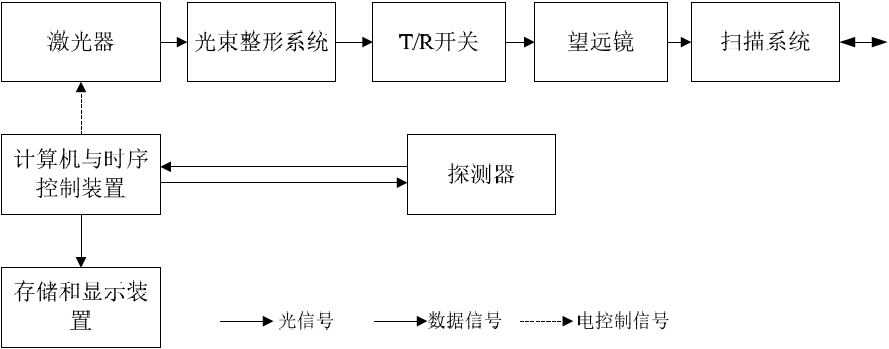
\includegraphics[width=0.7\linewidth]{figure/Chapter2/单稳系统的结构框图}
			\caption{单稳系统的结构框图}
			\label{fig:单稳系统的结构框图}
		\end{figure}
\end{itemize}

\subsection{光束整形} % Subsection 3.2	光束整形

\paragraph{光束整形}通过整形器控制出射激光的指向、方位信息、光束排布状况、束宽等参数,使其形成一定的排布规律,便于检测与分析。

激光器中的光学谐振腔无论是什么形状,其电磁场均具有一定的振荡频率和一定的空间分布,被称为\textit{腔的模式},用$ \mathrm{TEM}_{mn} $表示。其中,$ m = n = 0 $的模称为\textit{基模}。基模场振幅均满足高斯分布,这时激光光束称为\textit{基模高斯光束}。很多情况下要求将基模高斯光束整形为柱状对称,具有平顶强度分布的光束。如图\ref{fig:光束整形}所示。
\begin{figure}[htbp]
	\centering
	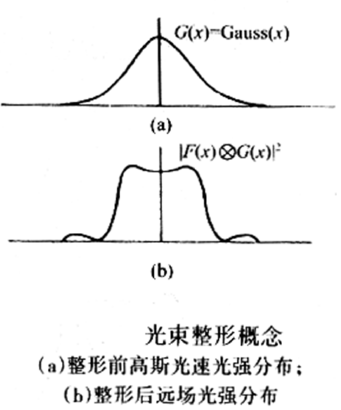
\includegraphics[width=0.3\linewidth]{figure/Chapter2/光束整形}
	\caption{光束整形}
	\label{fig:光束整形}
\end{figure}

\paragraph{光束整形的方法}\textit{衍射光栅}是光束整形的方法之一。光束整形器的能量色散元件由透明二元衍射光栅构成。选择合适的光栅周期和刻线相位调制深度,就可以达到所要求的整形效果。

\subsection{激光扫描} % Subsection 3.3	激光扫描

\paragraph{激光扫描}在光束整形之后,采用某种技术使激光束发生偏转,实现对某区域的目标进行扫描。

\paragraph{激光扫描技术的分类}
\begin{itemize}
	\item \textbf{高惯性扫描}
		\begin{itemize}
			\item 机械技术或反射镜棱镜技术
			\item 主要靠反射镜或棱镜的旋转实现扫描
		\end{itemize} % 高惯性扫描
	\item \textbf{低惯性扫描}
		\begin{itemize}
			\item 电光棱镜的梯度扫描
			\item 振动反射镜的非梯度扫描
			\item 增益控制或损耗控制的内腔式扫描
		\end{itemize}
\end{itemize} % 激光扫描技术的分类

\paragraph{衍射光学元件(DOE)}可替代旋转平面反射镜或棱镜,省去了机械转动部件,减少了折射元件数量,能对任意非球面误差进行校正。如图\ref{fig:衍射光学元件}所示。
\begin{figure}
	\centering
	\subfloat[衍射光学元件的衍射]{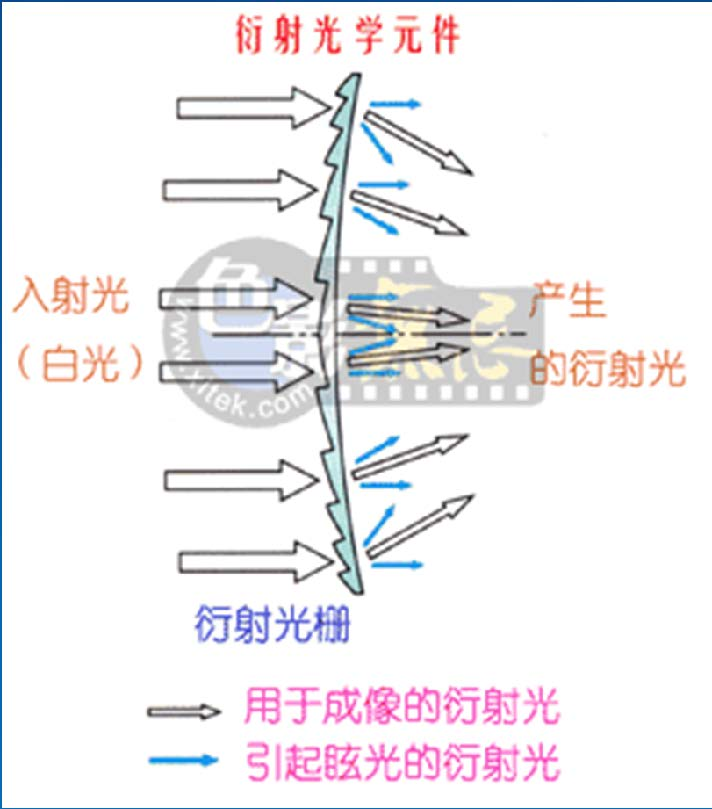
\includegraphics[height=4cm]{figure/Chapter2/衍射光学元件的衍射}}\quad
	\subfloat[DOE物镜后的区场扫描示意图]{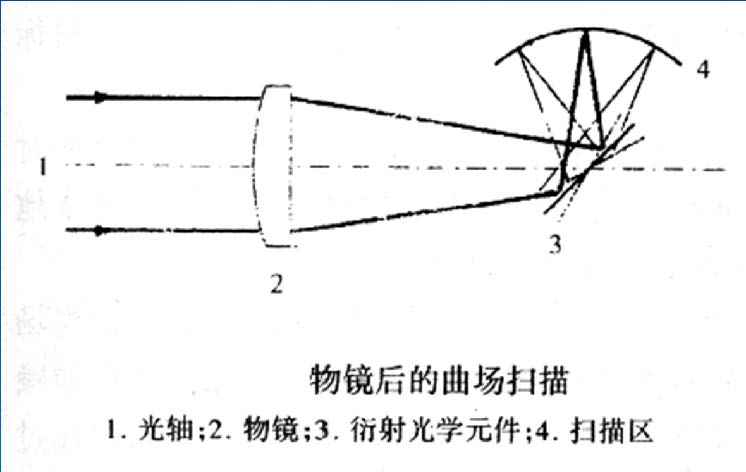
\includegraphics[height=4cm]{figure/Chapter2/DOE物镜后的区场扫描示意图}}
	\caption{衍射光学元件}
	\label{fig:衍射光学元件}
\end{figure}

\subsection{信号接收的探测技术} % Subsection 3.4	信号接收的探测技术
\paragraph{直接探测}将接收到的激光能量聚焦到光敏元件上,产生与入射光功率成正比的电压或电流。与传统的光学接收系统原理基本上相同。
\paragraph{相干探测}探测器接收目标回波信号和某一参考波的相干混合波信号,按照参考波的辐射源及其特性的不同进行探测。分为外差探测,零拍探测和多频外差探测等。
\begin{enumerate}
	\item \textit{外差探测}:
		一般外差探测激光雷达系统由一台连续工作的激光器作为独立辐射源发出参考波,称为\textit{本地振荡器}。
		系统接收到的回波信号与来自本地振荡器的参考信号混合之后,由混频器输出的光束聚焦到探测器上然后再进行信号处理。原理如图\ref{fig:外差探测}所示。
		\begin{figure}[htbp]
			\centering
			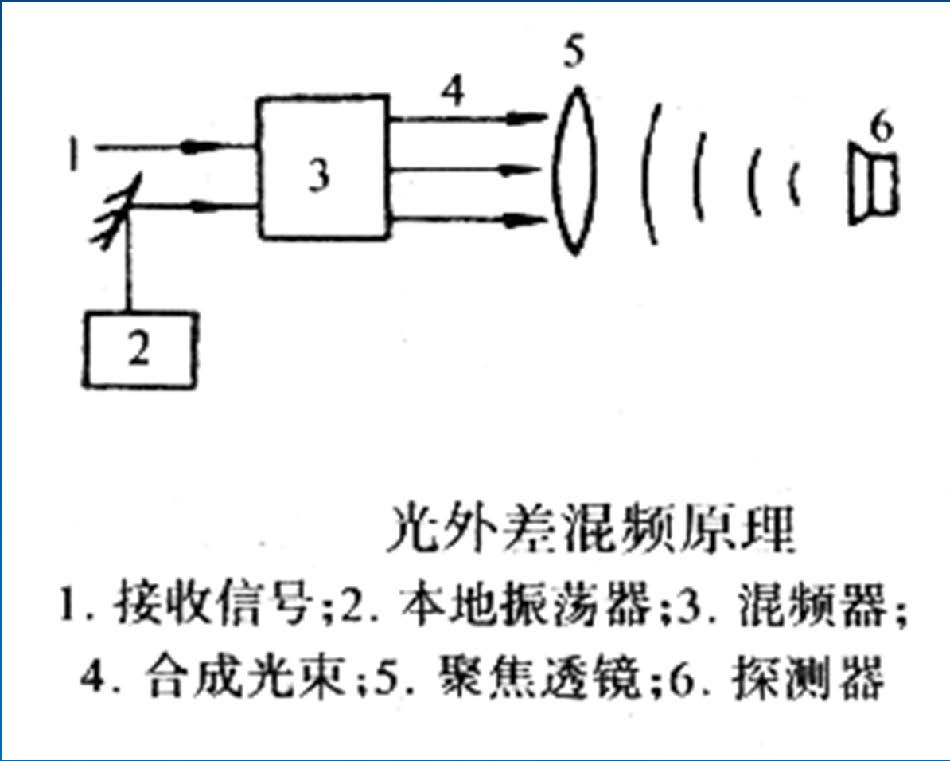
\includegraphics[width=0.5\linewidth]{figure/Chapter2/外差探测}
			\caption{外差探测原理}
			\label{fig:外差探测}
		\end{figure}
	\item \textit{零拍探测}:
		本地振荡信号是来自激光发射源的部分激光辐射,不需要另一个激光源。
		零拍激光雷达比普通外差激光雷达结构更简单,可靠性也更好。
		原理如图所示。
		\begin{figure}[htbp]
			\centering
			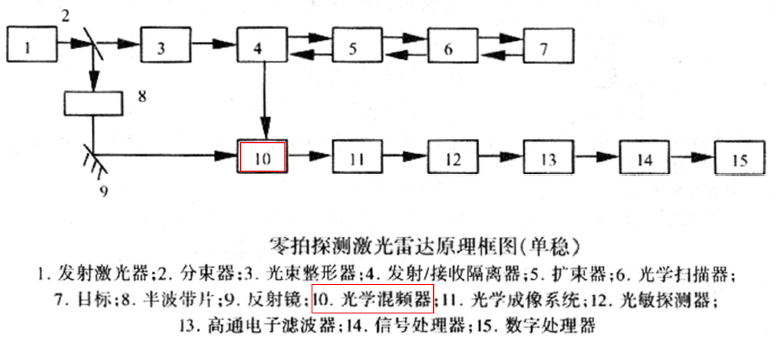
\includegraphics[width=0.7\linewidth]{figure/Chapter2/零拍探测}
			\caption{零拍探测}
			\label{fig:零拍探测}
		\end{figure}
	\item \textit{多频外差探测}:
		目标与激光雷达的相对运动产生接收信号的多普勒(Doppler)频移,可以提供有关目标的非常精确的信息;
		这要求外差探测接收器具有很宽的频带,以覆盖回波信号的频率和外差探测信号频率;
		但增加带宽会提高噪声水平,降低探测概率,解决这一问题的办法是采用三频外差系统。
		
		\textit{三频外差探测}:激光发射有两个独立辐射源,两束激光沿同一光轴向目标传播,经运动目标产生多普勒频移后返回接收器,两个反射信号与本地振荡器信号混频,成像在光敏探测器上。原理如图\ref{fig:三频外差探测系统示意图}所示。
		\begin{figure}[htbp]
			\centering
			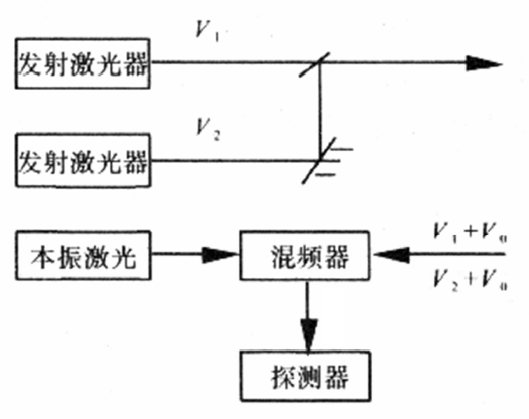
\includegraphics[width=0.5\linewidth]{figure/Chapter2/三频外差探测系统示意图}
			\caption{三频外差探测系统示意图}
			\label{fig:三频外差探测系统示意图}
		\end{figure}
\end{enumerate} % 相干探测的分类

\paragraph{接收孔直径}
\begin{itemize}
	\item 在相干探测激光雷达中,系统的有效接收孔径受散斑现象\footnote{被激光照明的物体,其表面呈现颗粒状结构。}的限制,不能任意扩大。
	\item 当接收孔径小于和等于散斑瓣的平均直径的情况下,接收功率是随接收孔的面积(孔径平方)线性增加;
	\item 在接收孔径增大,大于散斑瓣平均直径的情况下,接收功率不再服从与接收孔径面积线性相关的规律,而是与孔径线性相关;
		这种信号采集效率的下降是接收孔面积增大、反射信号相干性变差的结果;
	
		当接收孔径大于散斑瓣的平均直径时,接收孔有效直径可以表示为
		\begin{equation}
		D = \sqrt{D_rd_s}
		\end{equation}
		其中,$ D_r $表示接收器孔径实际大小,$ d_s $表示散斑瓣直径。
\end{itemize}

\section{激光信号的大气衰减}

\paragraph{激光的大气干扰}两次通过大气,不可避免受到干扰。由于激光光束波长较短,干扰主要有
\begin{itemize}
	\item 大气对它的吸收和散射作用较强,因此大气穿透能力较差。
	\item 大气中雨滴、尘埃、雾、霾等对激光的干扰作用大。
\end{itemize} % 激光的大气干扰

\paragraph{激光大气干扰的表现}
\begin{itemize}
	\item \textbf{衰减}:气体分子和气溶胶粒子、尘埃、雾、雨等的吸收和散射。
	\item \textbf{折射}:由于大气密度分布不均匀,导致激光沿光路产生折射。
	\item \textbf{其他}:大气湍流,导致光束扩展和漂移;大气吸收,引起光束相位变化。
\end{itemize} % 激光大气干扰的表现

\paragraph{激光雷达的性能}
\begin{itemize}
	\item 激光雷达的性能是与激光在大气中的传播特性密切相关的。
	\item 激光的传播特性主要与大气吸收、散射和折射的效应有关。
	\item 要充分发挥激光雷达的效能,就应充分了解激光的大气传播特性,寻找避免或克服大气效应的措施,减少大气衰减,并根据对激光在大气中的传播的规律,仔细选择激光工作波长以及激光工作方式,保证激光光束具有较高的透过率。
\end{itemize}

\subsection{大气衰减效应} % Subsection 4.1	大气衰减效应

\paragraph{布格埃—朗伯特定律}光束传播路径上大气均匀或分层均匀的情况下,目标处的光强可用布格埃—朗伯特定律描述:
\begin{equation}
I(\lambda,z) = I(\lambda,0)e^{-\sigma(\lambda)z}
\end{equation}
式中,$ z $为传播距离,$ I(\lambda,0) $、$ I(\lambda,z) $分别是波长为$ \lambda $的激光光束的初始光强和在距光源$ z $处的光强,$ \sigma(\lambda) $是与波长有关的衰减系数。

\paragraph{大气透过率}当激光束没有出现非线性效应时,大气透过率可以表示为
\begin{equation}
\tau(\lambda) = \exp\left\lbrace -\int_{0}^{L}\sigma(\lambda)\diff r \right\rbrace 
\end{equation}
其中$ L $是传播距离。对于水平平均光程,透过率可以写成
\begin{equation}
\tau(\lambda) = \exp\left\lbrace - \sigma(\lambda)L \right\rbrace
\end{equation}

\paragraph{总的衰减系数}
\begin{equation}
\sigma(\lambda) = \sigma_m + K_m + \sigma_a + k_a
\end{equation}
其中,$ \sigma_m $为分子散射系数,$ K_m $为分子吸收系数,$ \sigma_a $为气溶胶散射系数,$ k_a $为气溶胶吸收系数。
\begin{enumerate}
	\item \textbf{大气分子吸收——吸收系数}
		\begin{enumerate}
			\item \textbf{线吸收}:与单色光波长相应的大气分子的吸收。吸收系数:
				\begin{itemize}
					\item 高度在20 km以内,主要由碰撞压力展宽决定:
						\begin{equation}
						K_{ml} = \dfrac{S}{\pi}\dfrac{r_L}{(v-v_0)^2 + r_L^2}
						\end{equation}
						式中,$ v $是激光的波数,$ v_0 $是激光谱线中心的波数,$ S $为谱线的积分强度,$ r_L $为洛伦兹线半宽度,$ \alpha_D = S \cdot r_D $。
					\item 高度60 km以上,主要由多普勒展宽决定:
						\begin{equation}
						K_{MD} = \dfrac{S}{\alpha_D}\left[\dfrac{\ln 2}{\pi}\right]^{\dfrac{1}{2}} e^{-\frac{\ln 2(v-v_0)^2}{r_D^2}}
						\end{equation}
						式中,$ r_D $是多普勒谱线半宽度,$ \alpha_D = S \cdot r_D $,
						\begin{equation}
						r_d = \dfrac{v_0}{c}\left[\dfrac{2\ln 2k_BT}{M}\right]^{\frac{1}{2}} = 3.58 \times 10^{-7} \left[\dfrac{T}{M}\right] ^ {\frac{1}{2}}
						\end{equation}
					\item 在20$ \sim $60 km高度上,两种形式的吸收同时发生作用。
				\end{itemize} % 线吸收的吸收系数
			\item \textbf{连续吸收}:大气窗口内的大气分子。其吸收特点:
				\begin{itemize}
					\item 是随着光频率连续缓慢变化的分子吸收
					\item 在没有吸收线或只有很弱吸收的波长上,连续吸收成为主要因素
				\end{itemize}
				根据Kneizys得出的水汽连续吸收经验公式:
				\begin{itemize}
					\item 对10.6 μm的\ce{CO2}激光,必须考虑水汽和\ce{CO2}的连续吸收。
					\item 对10.6 μm的YAG激光,其连续吸收可以不加考虑。
				\end{itemize}
				在大气窗口内,水汽的连续吸收必须十分注意的。
		\end{enumerate} % 大气分子吸收——吸收系数
	\item \textbf{大气分子的散射}
		\begin{itemize}
			\item \textbf{瑞利散射}——大气分子。在光的波长远远大于大气中粒子之时, 大气散射表现为瑞利散射,散射系数的经验公式为
				\begin{equation}
				\sigma_m = 2.677 \times 10^{-17} \symrm{PV}^4/\symrm{T}
				\end{equation}
				其中,$ v $为波数。
			\item \textbf{米氏散射}——雨滴、雾滴、霾等粒子。当大气微粒直径很大,与激光波长可比拟之时大气散射服从米氏散射规律,一般说来,米氏散射是气溶胶散射。气溶胶粒子的总衰减系数近似表示:
				\begin{equation}
				\sigma_T = \sigma_a \sigma_m = \dfrac{3.912}{V_M} \left[\dfrac{0.55}{\gamma_{um}}\right]^b
				\end{equation}
				\begin{itemize}
					\item $ V_M $是能见度,即人眼可以辨别目标的最大距离。
					\item $ b $与能见度相关,
						\begin{itemize}
							\item 在一般条件下,$ V_M $为6$ \sim $20 km,$ b=1.3 $。
							\item 能见度特别好,$ V_M > $20 km时,$ b=1.6 $。
							\item 能见度小于6 km时,$ b = 0.585 $。 
						\end{itemize} % b
				\end{itemize} % 米氏散射
		\end{itemize} % 大气分子的散射
		总体说来, 大气分子和气溶胶的散射系数服从高度的负指数规律:随着高度的增加,散射系数很快减小。
		\begin{itemize}
			\item 在5 km以上——气溶胶散射系数与地面相比一般相差一个量级以上。
			\item 接近地面和低空中——气溶胶散射是主要的。
			\item 高空——分子散射与气溶胶散射的效果相当。
		\end{itemize}
\end{enumerate} % 衰减影响因素

\subsection{大气折射效应} % Subsection 4.2	大气折射效应

\paragraph{大气折射效应}激光通过大气时因不同的折射率造成光程增加,传播路径弯曲。

\paragraph{折射率}大气密度随着高度不同而变化,在不同的高度上大气对光的折射率不相同。大气折射率$ n $与激光波长$ \lambda $、空气的温度$ T $、湿度$ e $、压强$ P $有关
\begin{equation}
n = 1 + N(\lambda,T,P,e)
\end{equation}
式中,$ N $为\textit{折射率模数},单位为$ 10^{-6} $,一般简化写成$ N = 0.79 \times \symrm{P/T} $

\section{激光雷达系统能量方程} % Section 5 激光雷达方程

\paragraph{激光雷达方程}激光雷达能量探测的基本数学模型;
激光雷达因与目标作用的机理不同,分为不同的类型,不同类型的激光雷达要用不同的激光雷达方程加以描述。

\paragraph{激光雷达方程的一般形式}
\begin{equation}\label{equ:激光雷达方程的一般形式}
P_r = \dfrac{\eta_o \rho T_a^2 A_r}{\pi R^2} \cdot \dfrac{A_i}{A_b}P_t
\end{equation}
式中,$ P_r $是激光雷达接收到的激光功率;$ P_t $是光学系统效率;$ \rho $是目标表面反射率,$ T_a $是单程大气透过率,$ A_r $是光学系统有效接触面积,$ R $是目标与激光雷达的距离;$ A_i $是目标被照面积(截面积);$ A_b $是目标处的光斑面积。
式\eqref{equ:激光雷达方程的一般形式}\textbf{适用于发射、接收位于同一处的激光雷达的各种应用情况。}

\paragraph{单脉冲稳频激光雷达}探测器所测得的目标,距离探测器$ R $到$ R+\diff R $,辐射源产生的波长间隔为$ [\lambda,\lambda + \diff \lambda] $的微分信号功率为
\begin{equation}
\diff P(\lambda,R) = I(\lambda,R,r)p(\lambda,R,r)\diff\lambda \diff R \diff A(R,r) 
\end{equation}
探测器所接收到的总信号功率则表示为
\begin{equation}
P(\lambda,R) = \int_{0}^{R}\diff R\int_{\Delta\lambda}\int I(\lambda,R,r)p(\lambda,R,r)\diff A(R,r)
\end{equation}
其中,$ p(\lambda,R,r) $取决于
\begin{itemize}
	\item 大气传输因子;
	\item 接收系统传输因子$ T_r(\lambda) $;
	\item 接收立体角$ \dfrac{A_0}{R^2} $;
	\item 接收视场与激光辐射照射面的重叠因子及在距离$ R $到$ R+\diff R $内回波到达探测器的概率$ p(R) $。
\end{itemize} % p(\lambda,R,r)取决于

% !TeX encoding = UTF-8
% !TeX spellcheck = en_US
% !TeX root = main.tex

%% Chapter03-机载LiDAR数据获取基本原理.tex
\chapter{机载LiDAR数据获取基本原理} %% Chapter 机载LiDAR数据获取基本原理

\paragraph{机载LiDAR系统工作原理}如图\ref{fig:机载LiDAR系统工作原理图}所示。
\begin{figure}[htbp]
	\centering
	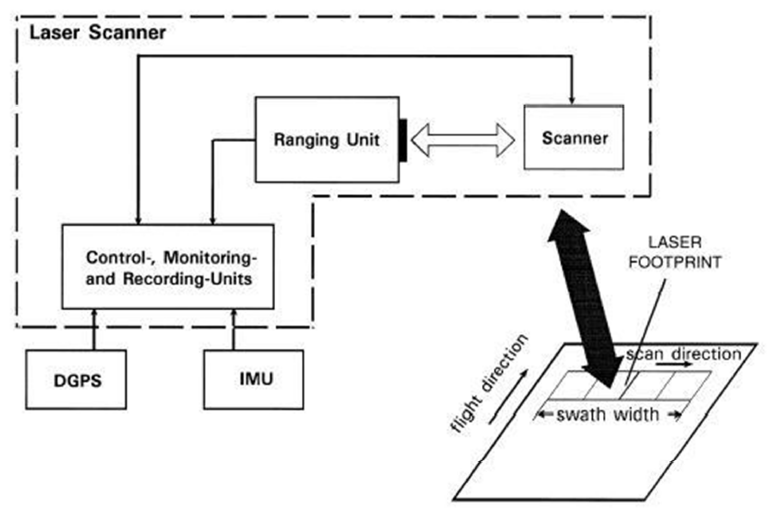
\includegraphics[width=0.7\linewidth]{figure/Chapter3/机载LiDAR系统工作原理图}
	\caption{机载LiDAR系统工作原理图}
	\label{fig:机载LiDAR系统工作原理图}
\end{figure}

图中,
\begin{itemize}
	\item \textit{激光测距单元}包括:激光发射器和接收机。
	\item 光学机械扫描装置:主动工作方式。
		\begin{itemize}
			\item 激光发射器产生激光,由扫描装置控制激光束发射出去的方向
			\item 扫描方向一般与飞机飞行方向垂直。
			\item 扫描宽度由\textit{扫描视场}(FOV,field of view)决定。
		\end{itemize}
	\item 发射和接收激光束的光孔是同一光孔,孔径一般为8$ \sim $15 cm,保证发射光路和接收光路是同一光路。
	\item 发射的激光束是一束很窄的光,发散度很小,形成的\textit{瞬时视场}(IFOV,instantaneons field of view)是由一个很小的角度确定的,一般为0.3 毫弧(mrad)到0.2 毫弧,激光束形成的一个照射角,照射在一小块地面。
	\item 接收机接收被反射回来的激光束后由记录单元进行记录。
\end{itemize}

\paragraph{关键技术}
\begin{itemize}
	\item 激光测距技术
	\item 全球定位系统技术
	\item 惯性测量系统技术
	\item 高性能二维扫描技术
\end{itemize}

\section{激光测距} %% Section	激光测距	========================================
\paragraph{机载LiDAR系统对测距仪的要求}
\begin{itemize}
	\item 精度高
	\item 功率高
	\item 体积小
	\item 波长合适
\end{itemize}

\paragraph{激光测距基本原理}测量激光往返目标所需要时间,然后通过光速$ c $(299792458 m/s)和大气折射系数计算出距离。如图\ref{fig:激光测距基本原理}所示。
\begin{figure}[htbp]
	\centering
	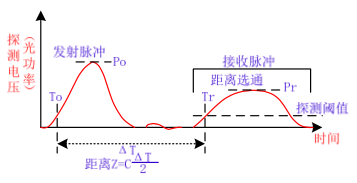
\includegraphics[width=0.7\linewidth]{figure/Chapter3/激光测距基本原理}
	\caption{激光测距基本原理}
	\label{fig:激光测距基本原理}
\end{figure}

\subsection{测距方式} % Subsection	测距方式	----------------------------------------
\paragraph{脉冲测距}
\begin{enumerate}
	\item \textbf{测距原理}:发射脉冲波,测量脉冲信号往返时间差,如图\ref{fig:脉冲测距原理}所示。距离为
		\begin{equation}
		R = \dfrac{1}{2}ct_L
		\end{equation}
		\begin{figure}[htbp]
			\centering
			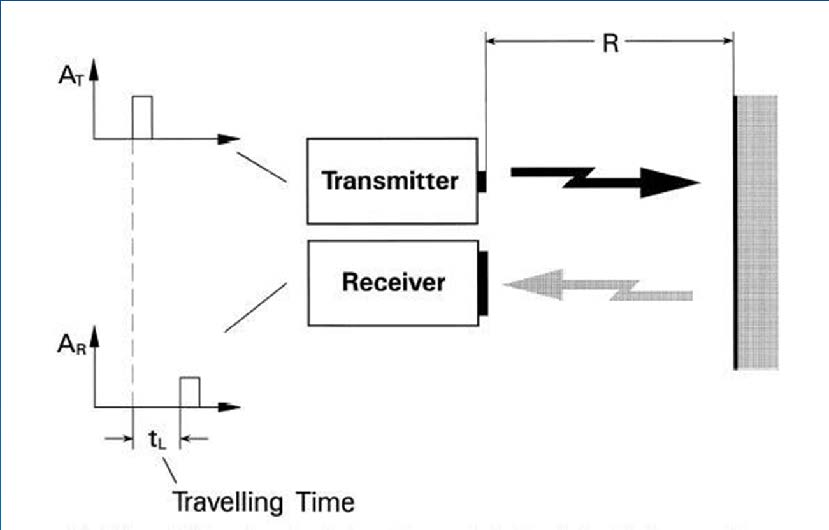
\includegraphics[width=0.5\linewidth]{figure/Chapter3/脉冲测距原理}
			\caption{脉冲测距原理}
			\label{fig:脉冲测距原理}
		\end{figure}
	\item \textit{测距分辨率}:在光束方向能够区分的两个物体的最小距离。
		\begin{equation}
		\Delta R = \dfrac{1}{2}c\Delta t_L
		\end{equation}
		实际上它是取决于$ \Delta t $,即计时器精度。
	\item \textit{最大测量距离}:采用激光器发射激光脉冲时要考虑,避免最远目标所反射的激光束还未返回就发射下一束激光。
	
		需要考虑可能的最大量测距离与最远的目标有关。
		\begin{equation}
		R_{\max} = \dfrac{1}{2}ct_{L_{\max}}
		\end{equation}
		
		\textit{脉冲发射频率}是指一秒钟内能发射多少次激光束,决定了相邻的两束脉冲的时间间隔,由此决定了最大量测距离。
	\item \textbf{脉冲激光测距仪的误差}:对于脉冲激光,计时器主要依脉冲的特殊点进行记录。
		实际脉冲并非一个完全的矩形波,一般事先确定一个阈值,当信号电压到达这一阈值时,计时器即开始记录,由阈值触发器电路控制,结束记录时也是如此。
		
		\textbf{计时误差}:如果所接收的激光幅值很低,电压值未调整到与发射时相同电压值,所记录时间就会过长!解决办法:
			\begin{itemize}
				\item 一般在记时器的前端安置一个放大器进行信号调整。
				\item 为避免因激光幅值变化造成记时错误,采用\textit{分数鉴别器},代替阈值鉴别器: 按信号峰值的比例系数作为记时参照常量。
			\end{itemize}
\end{enumerate} % 脉冲测距

\paragraph{连续波相位差测距}
\begin{enumerate}
	\item \textbf{基本原理}:发射连续波,测量往返连续波的相位差。基本原理如图\ref{fig:连续波相位差测距原理}所示。
		
		\begin{figure}[htbp]
			\centering
			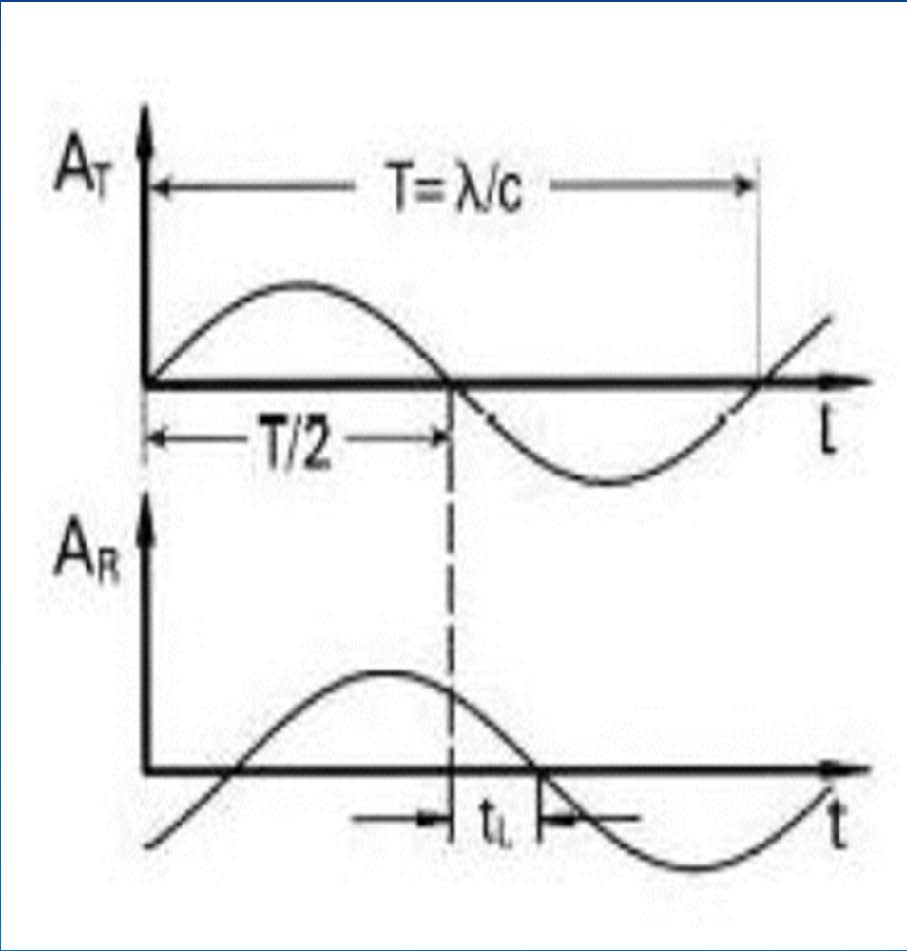
\includegraphics[width=0.5\linewidth,height=0.2\textheight]{figure/Chapter3/连续波相位差测距原理}
			\caption{连续波相位差测距原理}
			\label{fig:连续波相位差测距原理}
		\end{figure}
		
		若在时间$ T $内的被接收的波与被发射波的相位差为$ \varphi $,则从发射到被接收所用时间为
		\begin{equation}
		t_L = \dfrac{\varphi}{2\cpi}\cdot T
		\end{equation}
		
		测量的距离为
		\begin{equation}
		R = \dfrac{1}{2}c \cdot \dfrac{\varphi}{2\cpi}\cdot T = \dfrac{\lambda}{4\cpi}\varphi
		\end{equation}
	
	\item \textbf{测距分辨率}:相位测距中能够准确测量的是一个周期以内的相位差,测距分辨率为
		\begin{equation}
		\Delta R = \dfrac{\lambda_{\text{short}}}{4\cpi}\varphi
		\end{equation}
	\item \textit{整周模糊度}:图中$ t_L $与接收信号与发射信号的相位差成正比。$ t_L $应表示为
		\begin{equation}
		t_L = \dfrac{\varphi}{2\cpi}T+nT
		\end{equation}
		式中,$ n $为激光从发射到接收所走过的距离中的整周数。由于激光波长以微米计,可见$ n $为一个很大的数。由于实际量测的相位差只在之内,实际计算目标到激光器的距离必须计算出整周数$ n $。
	\item \textbf{多测尺频率}:
		若用单一频率测距时是无法确定整周模糊度的值 ,即测距仪存在多值性问题,要解决这一问题,必须采用几个测尺频率测定同一距离。方法:
		\begin{itemize}
			\item 直接多测尺频率:适用于短距离;
			\item 间接多测尺频率:适用于中长距离;
		\end{itemize} % 多测尺频率
	\item \textbf{最大量测距离}:由于相位差的最大量测值为$ 2\cpi $,有
		\begin{equation}
		R_{\max} = \dfrac{1}{4\cpi}\lambda\varphi = \dfrac{\lambda_{\text{long}}}{2}
		\end{equation}
		\begin{itemize}
			\item \textit{最大不模糊距离}:能够准确测量的最大距离,称为最大不模糊距离。
			\item \textbf{双频观测系统}:在采用多频率系统时,由不同频率所对应的波长可兼顾较高的测距分辨率和较大的测量距离。很明显,由最短波长确定了较高的测距分辨率和精度,最长波长确定了最大不模糊距离。
		\end{itemize}
\end{enumerate} % 连续波相位差测距

\paragraph{结论}
\begin{itemize}
	\item 无论是脉冲激光还是连续波激光,在其它条件不变的情况下,最大测距与反射率的平方根和激光功率的平方根成正比。
	\item 要获得较好的测距效果
		\begin{itemize}
			\item \textbf{气候条件}:大气条件十分重要,干、冷和透明的大气条件下,效果最好;
			\item \textbf{时间条件}:夜间最好,最坏的情况是白天阳光强烈;
			\item \textbf{波段选择}:选择大气透过率高的波段;
		\end{itemize}
\end{itemize}

\subsection{测距精度和信噪比} % Subsection	测距精度与信噪比	----------------------------------------
\paragraph{测距精度和信噪比的关系}激光测距系统的测距精度与测距信号的信噪比的平方根成反比,信噪比愈高,测距精度也越高。
\begin{equation}
\sigma \sim \dfrac{1}{\sqrt{S/N}}
\end{equation}

\paragraph{信噪比} 
\begin{itemize}
	\item 信噪比取决于很多因素,如:接收信号功率、信号带宽、背景辐射、探测器响应灵敏度、放大器噪声等。如图\ref{fig:信号参量之间的关系以及对信噪比的影响}所示。
		\begin{figure}
			\centering
			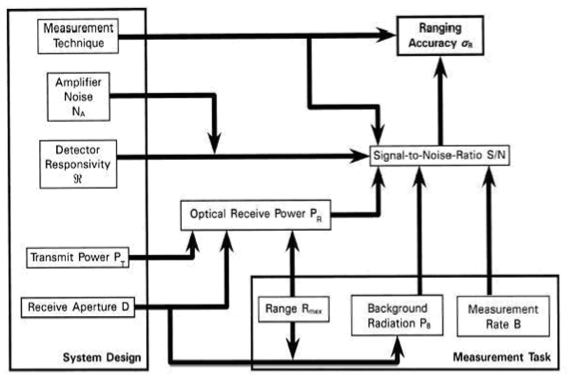
\includegraphics[width=0.7\linewidth]{figure/Chapter3/信号参量之间的关系以及对信噪比的影响}
			\caption{信号参量之间的关系以及对信噪比的影响}
			\label{fig:信号参量之间的关系以及对信噪比的影响}
		\end{figure}
	\item \textbf{信噪比简化}
		\begin{equation}
		S/N = \dfrac{\text{光电二极管电流中的信号功率}}{\text{光电二极管和放大器中的热噪声}}
		\end{equation}
\end{itemize}

\paragraph{两种测距方式的精度}
由于测距精度和信噪比成反比,如果脉冲测距时噪声带宽为$ B_{\text{pulse}} $,相位差测距时噪声带宽为$ B_{\text{cw}} $,则下述关系式成立:
\begin{align}
\sigma_{R_{\text{pulse}}} & \sim \dfrac{c}{2}t_{\text{rise}}\dfrac{\sqrt{B_{\text{pulse}}}}{P_{R_{\text{peak}}}} \\
\sigma_{R_{\text{cw}}} & \sim \dfrac{\lambda_{\text{short}}}{4\cpi}\dfrac{\sqrt{B_{\text{cw}}}}{P_{R_{\text{av}}}}
\end{align}
式中,$ P_{R_{\text{peak}}} $表示脉冲接收功率峰值,$ P_{R_{\text{av}}} $表示连续波接收功率平均值。

假定对同一目标进行量测,可以用发射功率代替接收功率,即以脉冲激光发射功率峰值$ P_{T_{\text{peak}}} $代替接收功率峰值$ P_{R_{\text{peak}}} $,以连续波发射功率平均值$ P_{T_{\text{av}}} $代替接收功率平均值$ P_{R_{\text{av}}} $。于是有:
\begin{equation}\label{equ:两种测距方式精度之比1}
\dfrac{\sigma_{R_{\text{pulse}}}}{\sigma_{R_{\text{cw}}}} \sim 2\cpi \dfrac{c}{\lambda}t_{\text{rise}} \dfrac{P_{T_{\text{av}}}}{P_{T_{\text{peak}}}} \sqrt{\dfrac{B_{\text{pulse}}}{B_{\text{cw}}}}
\end{equation}
假定
\begin{equation}
t_{\text{rise}} \sim \dfrac{1}{B_{\text{pluse}}}
\end{equation}
式\eqref{equ:两种测距方式精度之比1}可以写为
\begin{equation}
\dfrac{\sigma_{R_{\text{pulse}}}}{\sigma_{R_{\text{cw}}}} \sim 2\cpi f \sqrt{\dfrac{t_{\text{rise}}}{B_{\text{cw}}}} \dfrac{P_{T_{\text{av}}}}{P_{T_{\text{peak}}}}
\end{equation}

\paragraph{现状}脉冲激光系统具有大功率、可远距离测距等特点,
目前市场上绝大多数为脉冲激光系统,很少有半导体连续波激光系统。
不过脉冲系统要达到很高的精度需要非常高的技术手段和复杂的处理方法。

\paragraph{测距误差}\textit{测距误差}是指测距仪的显示结果与实际距离之差。
\begin{enumerate}
	\item \textbf{测距误差来源}:噪声、脉冲宽度和幅度、电光系统的延迟以及时间测量单元中基准振荡频率的稳定性。
	\item \textbf{脉冲激光测距仪的误差}
		\begin{itemize}
			\item \textbf{系统误差}:
				\begin{itemize*}
					\item 计数器误差
					\item 大气折射误差
					\item 光电延迟误差
				\end{itemize*}
			\item \textbf{随机误差}:
				\begin{itemize*}
					\item 噪声误差
					\item 距离误差
					\item 漂移误差
				\end{itemize*}
		\end{itemize} % 脉冲激光测距仪的误差
	\item \textbf{连续波激光测距仪测距误差}
		\begin{itemize}
			\item \textbf{固定误差}:
				\begin{itemize*}
					\item 数字测相误差
					\item 幅相误差
					\item 照准误差
				\end{itemize*}
			\item \textbf{比例误差}:
				\begin{itemize*}
					\item 真空光速误差
					\item 大气折射率误差
					\item 测尺频率误差
				\end{itemize*}
		\end{itemize} % 连续波激光测距仪测距误差
	\item \textbf{影响LiDAR测距精度的因素还有}
		\begin{itemize}
			\item 激光功率
			\item 光束发散度
			\item 目标反射特性
			\item 探测器灵敏度
			\item 飞行高度
			\item 飞机姿态
		\end{itemize} % 影响LiDAR测距精度的因素还有
\end{enumerate} % 测距误差

\subsection{功率} % Subsection	功率	----------------------------------------
由于LiDAR系统是在空中对地面进行扫描的,它需要有很高的工作功率,这样才能使激光束的能量尽可能大,经过长距离的大气损耗 和目标吸收等能量损失后,回到探测器时能够有足够的能量,使得探测器能够对光束进行记录。

\paragraph{峰值功率与平均功率}
对于脉冲测距系统,激光能量为:
\begin{equation}
E_{\text{pluse}} = P_{T_{\text{peak}}} t_{\text{pulse}}
\end{equation}
式中,$ t_{\text{pulse}} $为脉冲宽度,$ P_{T_{\text{peak}}} $为发射功率峰值。
	
如果脉冲频率为$ f_{\text{pluse}} $,则平均功率为
\begin{equation}
P_{T_{\text{av}}} = E_{\text{pluse}}f_{\text{pluse}}
\end{equation}

联立求解,得
\begin{equation}
P_{T_{\text{peak}}} = \dfrac{E_{\text{pluse}}}{t_{\text{pulse}}} = \dfrac{P_{T_{\text{av}}}}{t_{\text{pulse}}f_{\text{pluse}}}
\end{equation}
尽管平均功率不大,脉冲激光测距能够产生很高的峰值功率。

\paragraph{发射功率与接受功率}
\begin{equation}
P_r = \rho \dfrac{M^2 A_r}{\cpi R^2} P_T
\end{equation}
式中,$ M $为大气透过率,$ \rho $为目标反射率,$ R $为目标到激光器的距离,$ A_r $为接收光孔截面积。

接受功率的特点:
\begin{itemize}
	\item LiDAR系统接收的功率只是发射功率的很小部分,必须采用非常灵敏的探测器接收信号 。
	\item 接收功率与距离平方成反比
		\begin{itemize}
			\item 激光束刚刚发射出来,由于空中的尘埃或其它的干 扰,会有一部分信号返回接收光路,即使这个部分非常小,也会被灵敏的探测器认为是目标的回波。
			\item 为了避免这种情况,需要采取\textit{近距离消除技术}(close-range suppression techniques)和其它方法。
		\end{itemize}
\end{itemize}

\subsection{体积} % Subsection	体积	----------------------------------------
由于LiDAR系统安装在空中平台上,飞机 的载重量和体积都是有限的,在有限的空间 中需要装载LiDAR设备、操作人员等。
因此,需要将LiDAR设备的体积和重量减小到最小, 这也要求测距仪的体积和重量都很小。

\subsection{波长} % Subsection	波长	----------------------------------------
\paragraph{选择波长的依据}
\begin{itemize}
	\item 大气窗口
	\item 背景光的区别
	\item 目标反射率
	\item 探测器灵敏度
	\item 人眼安全
\end{itemize}

\paragraph{常见LiDAR系统的激光波长} 如表\ref{tab:常见LiDAR系统的激光波长}所示。

\begin{table}[!htbp]
	\centering
	\begin{tabular}{|c|c|}
		\hline
		              系统              &       激光波长       \\ \hline
		\multirow{2}{*}{Leica ALS50II} &  790$ \sim $820  \\ \cline{2-2}
		                               & 1050$ \sim $1060 \\ \hline
		        Optech 3100EA          &       1064       \\ \hline
		      TopoSys FALCON II        &       1560       \\ \hline
		        Riegl LMS-Q560         &       1500       \\ \hline
	\end{tabular}
	\caption{常见LiDAR系统的激光波长}
	\label{tab:常见LiDAR系统的激光波长}
\end{table}

\section{全球定位系统技术} %% Section	全球定位系统技术	========================================
\paragraph{全球定位系统}\textit{全球定位系统}(GPS, Global Position System)是一种利用人造地球卫星进行点位测量导航的技术。
全称是NAVSTAR GPS(NAVigation Satellite Timing And Ranging Global Positioning System)。

\paragraph{GPS定位原理}利用\textbf{测距交会确定点位}。由于用户接受机使用的时钟与卫星星载时钟不可能总是同步,所以除了用户的三维坐标$ (x,y,z) $外,还要引入一个关于卫星与接收机之间的时间差作为未知数$ \delta T $。所以如果想知道解收机所处的位置,至少要能接收到4个卫星的信号。

\paragraph{GPS的组成}
\begin{itemize}
	\item \textbf{空间部分}:GPS卫星星座。如图\ref{fig:GPS星座}所示。
		\begin{itemize}
			\item 由21颗工作卫星和3颗备用卫星组成。
			\item 均匀分布在六个相互夹角为$ 60^{\circ} $的轨道平面内。
			\item GPS卫星用L波段两种频率的无线电波(1575.42 MHz和 1227.6 MHz)向用户发射导航定位信号,同时接收地面发送的导航电文以及调度命令。
		\end{itemize}
		
		\begin{figure}[htbp]
			\centering
			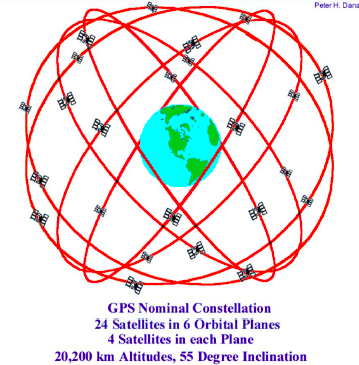
\includegraphics[width=0.5\linewidth]{figure/Chapter3/GPS星座}
			\caption{GPS星座}
			\label{fig:GPS星座}
		\end{figure}
	\item \textbf{地面控制部分}:地面监控系统。
		包括位于美国科罗拉多的主 控站以及分布全球的三个注入站和五个监测站组成,实现对GPS卫星运行的监控。
		主要任务是采集数据(对空中卫星进行连续观测),推算编制各卫星的星历、卫星钟差及大气层的修正参数等,并将这些数据发送到卫星上。
	\item \textbf{用户设备部分}:GPS信号接收机。用来捕获GPS卫星发射的信号,并进行处理,
		根据信号到达接收机的时间,确定接收机到卫星的距离,并最终确定接收机的精确位置。
\end{itemize} %. GPS的组成

\paragraph{GPS的优点}
\begin{itemize}
	\item 观测站之间无需通视
	\item 定位精度高
	\item 操作简便
	\item 全天候作业
	\item 实时定位速度快
	\item 抗干扰性能好,保密性强
\end{itemize}

\paragraph{GPS定位分类}
\begin{enumerate}
	\item \textbf{按定位方式}
		\begin{itemize}
			\item \textit{单点定位(绝对定位)}:采用一台接收机进行定位的模式。只能采用伪距观测量进行概略导航定位,定位精度较差。
			\item \textit{差分定位(相对定位)}:差分GPS(Differential Global Position System,DGPS)
				在用户接收机附近设置一个坐标已知的差分基准站, 连续接收GPS导航信号,将测得的位置或距离数据与已知的位置、距离数据进行比较,
				确定误差,得出改正值,然后将改正数发播给覆盖区域内的用户,用以改正用户的定位结果。
		\end{itemize} % 按定位方式
	\item \textbf{根据定位所采用的观测值} 
		\begin{itemize*}
			\item 测距码伪距GPS定位
			\item 载波相位GPS定位
		\end{itemize*}
	\item \textbf{根据获取定位结果的时间} 
		\begin{itemize*}
			\item 实时GPS定位
			\item 非实时GPS定位
		\end{itemize*}
	\item \textbf{根据定位时接收机的运动状态} 
		\begin{itemize*}
			\item 动态GPS定位
			\item 静态GPS定位
		\end{itemize*}
\end{enumerate}

\paragraph{GPS精度影响因素}
\begin{itemize}
	\item 接收机公有的误差
	\item 传播延迟误差
	\item 接收机固有的误差
\end{itemize}
DGPS技术可以完全消除第一部分误差,大部分消除第二部分误差(取决于基准站和流动站之间的距离)。

\paragraph{LiDAR系统的GPS技术}
LiDAR系统要求很高的定位精度,采取的是载波相位 差分GPS技术,又称为RTK(Real Time Kinematic)技术,
建立在实时处理两个测站的载波相位观测值的基础上,它能实时提供观测点的三维坐标,可以达到厘米级的高精度。

由于涉及到测定遥感器投影中心的位置方位元素,在机载激光雷达系统中,GPS动态定位的精度成为影响系统精度的主要因素。
一般而言,LiDAR系统上使用的载 波相位差分GPS定位精度在5 cm$ \sim $10 cm。

\paragraph{LiDAR系统中GPS的作用}
\begin{itemize}
	\item 确定成像时刻系统中心的地理坐标
	\item 提供相关数据给姿态测量装置,提高测定姿态角的测角精度
	\item 提供导航控制数据
\end{itemize}

\section{惯性测量系统技术} %% Section	全球定位系统技术	========================================
\subsection{惯性导航系统} % Subsection	惯性导航系统	----------------------------------------
\paragraph{基本原理}
\textit{惯性导航系统}(Inertial Navigation System, INS),利用陀螺和加速度计等惯性元件测量运行体在运动过程中的旋转角速度和加速度,计算得到运动体的相对位置、速度和姿态等导航参数。
结构如图\ref{fig:惯性导航系统结构}所示。

\begin{figure}[htbp]
	\centering
	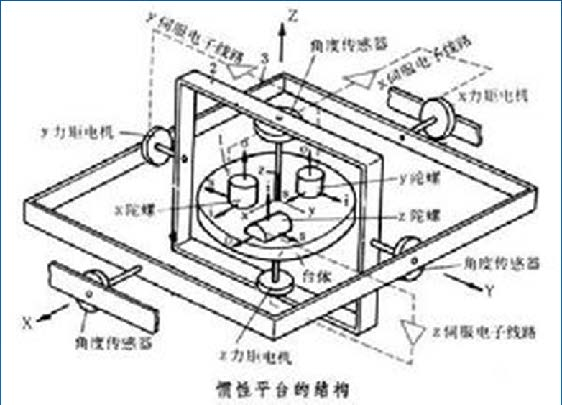
\includegraphics{figure/Chapter3/惯性导航系统结构}
	\caption{惯性导航系统结构}
	\label{fig:惯性导航系统结构}
\end{figure}

\paragraph{作用}可以用于定位、测速、输出姿态信息,以及测定重力异常和垂线偏差、相对大地水准面起伏等。

\paragraph{惯性测量单元} 惯性导航系统中负责姿态测定的陀螺和加速度计等惯性元件总称为\textit{惯性测量单元}(Inertial Measurement Unit, IMU),它是INS的核心部件。IMU通常由三个加速度计和三个陀螺、数字电路和CPU组成的。

\subsection{IMU与DGPS组合定位技术} % Subsection	IMU与DGPS组合定位技术	----------------------------------------
\paragraph{DGPS技术的特点}
\begin{itemize}
	\item \textbf{优点}:使用方便、成本低廉,可量测传感器的位置和速率,高精度、误差不随时间积累。
	\item \textbf{缺点}:动态性能差、数据输出频率低(易受到干扰而失锁),无法量测瞬间的快速变化,没有姿态量测功能等。
\end{itemize}

\paragraph{IMU技术的特点}
\begin{itemize}
	\item \textbf{优点}:姿态量测功能,具有完全自主、无信号传播,既能定位、测速,又可快速量测传感器瞬间的移动,输出姿态信息。
	\item \textbf{缺点}:位误差随着时间迅速积累增长,每次使用前初始对准时间长,不能长时间单独工作,必须不断加以校准。
\end{itemize}

\paragraph{POS系统}GPS技术+IMU技术
\begin{itemize}
	\item 提高了定位精度
	\item 增强了系统可靠性
	\item 部分解决了采样频率低的问题
\end{itemize}

\section{高性能二维扫描技术} %% Section	全球定位系统技术	========================================
\subsection{机载LiDAR系统四种典型的扫描方式} % Subsection	机载LiDAR系统四种典型的扫描方式	----------------------------------------
\begin{enumerate}
	\item \textit{摆镜扫描}:通过电机带动反射镜反复摆动一定的角度,实现激光束在地面的扫描。扫描原理和脚点形状如图\ref{fig:摆镜扫描}所示。
		\begin{figure}[htbp]
			\centering
			\subfloat[摆镜扫描原理]{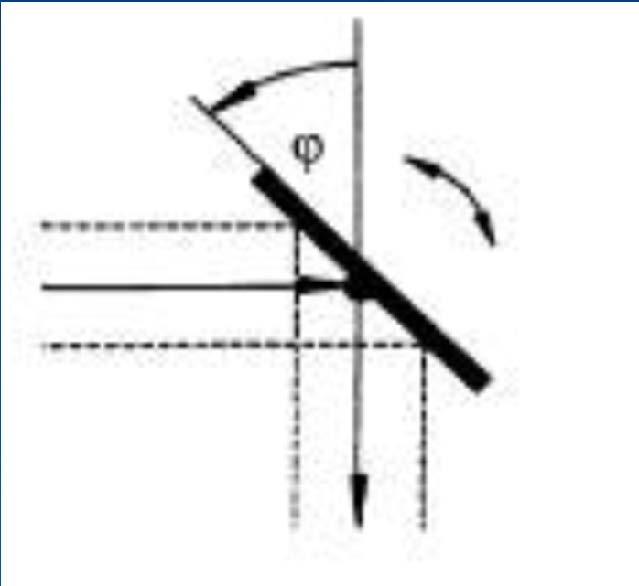
\includegraphics[height=3cm]{figure/Chapter3/摆镜扫描1}}\quad
			\subfloat[摆镜扫描结构]{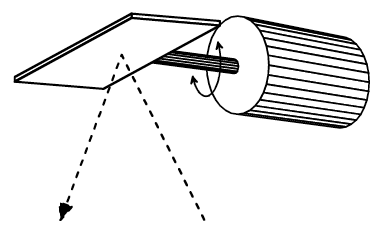
\includegraphics[height=3cm]{figure/Chapter3/摆镜扫描2}}\quad
			\subfloat[摆镜扫描脚点]{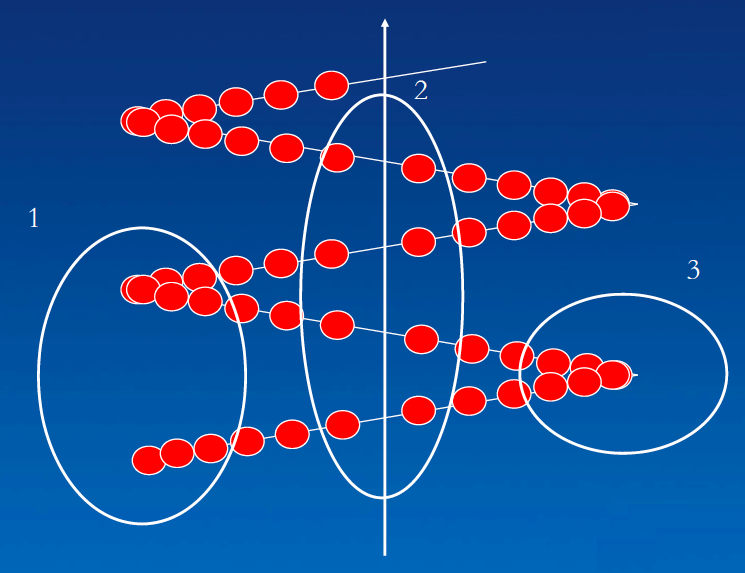
\includegraphics[height=3cm]{figure/Chapter3/摆镜扫描_脚点}}
			\caption{摆镜扫描}
			\label{fig:摆镜扫描}
		\end{figure}
	\item \textit{旋转棱镜扫描}:通过电机带动多面棱镜旋转,由于镜面的位置在不断变化,导致反射光束的方向在一定的范围内往复变化,从而实现激光束在地面的扫描。如图\ref{fig:旋转棱镜扫描}所示。
		\begin{figure}[htbp]
			\centering
			\subfloat[旋转棱镜扫描原理]{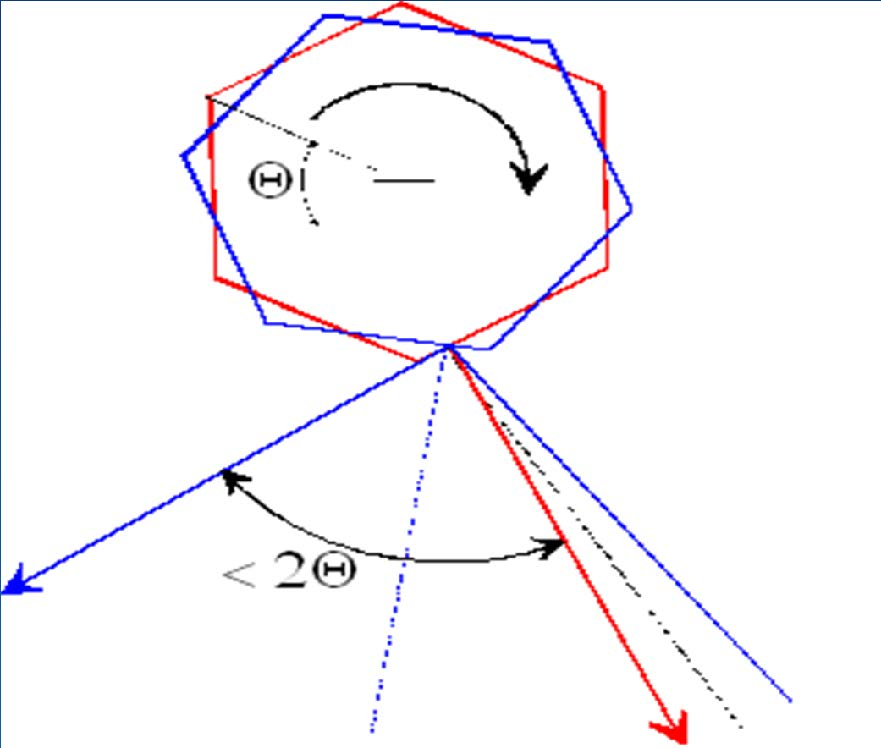
\includegraphics[height=3cm]{figure/Chapter3/旋转棱镜扫描原理}}\quad
			\subfloat[旋转棱镜扫描脚点形状]{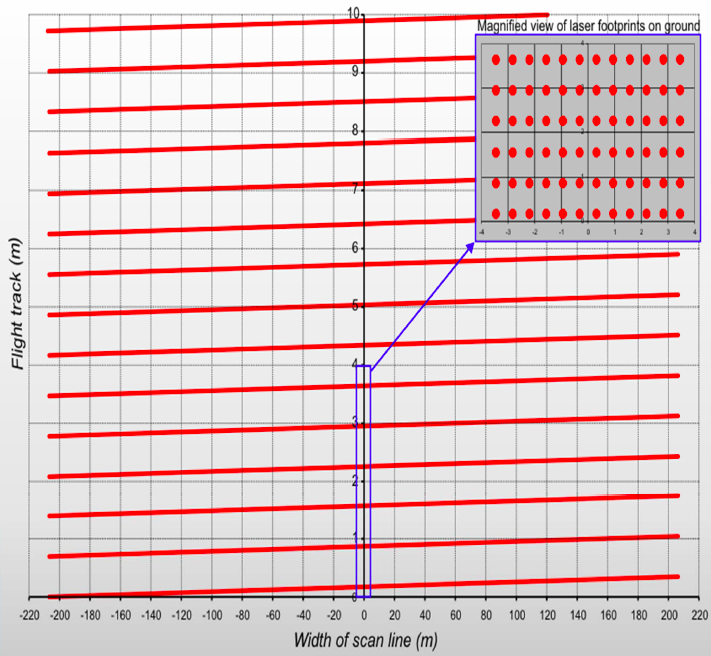
\includegraphics[height=3cm]{figure/Chapter3/旋转棱镜扫描脚点形状}}
			\caption{旋转棱镜扫描}
			\label{fig:旋转棱镜扫描}
		\end{figure}
	\item \textit{椭圆扫描}:旋转一周后在地面形成椭圆扫线。如图\ref{fig:椭圆扫描}所示。
		\begin{figure}[htbp]
			\centering
			\subfloat[椭圆扫描示意图]{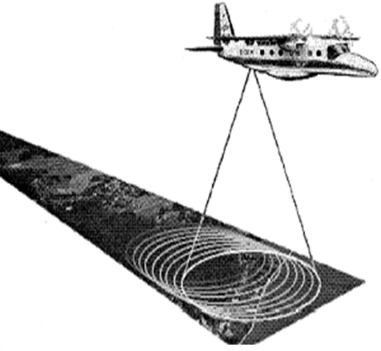
\includegraphics[height=3cm]{figure/Chapter3/椭圆扫描1}}\quad
			\subfloat[椭圆扫描原理]{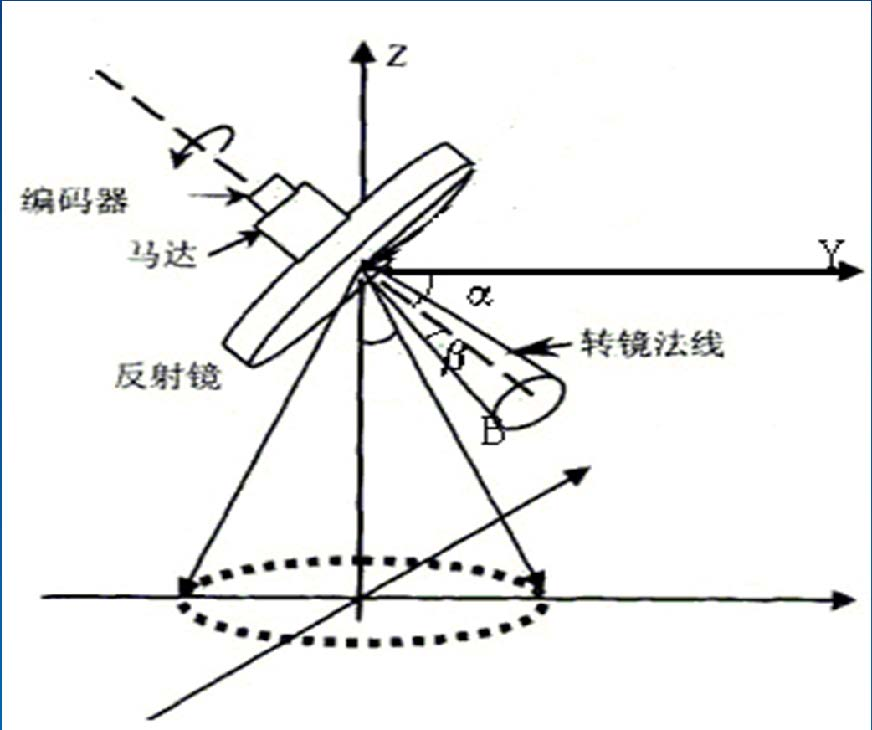
\includegraphics[height=3cm]{figure/Chapter3/椭圆扫描2}}\quad
			\subfloat[椭圆扫描脚点形状]{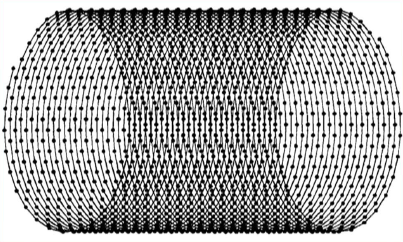
\includegraphics[height=3cm]{figure/Chapter3/椭圆扫描脚点形状}}
			\caption{椭圆扫描}
			\label{fig:椭圆扫描}
		\end{figure}
	\item \textit{光纤扫描}:如图\ref{fig:光纤扫描}所示。目前仅TopoSys激光系统采用光纤扫描仪。目前已有128根光纤组,256根光纤组将可以实现。
		\begin{figure}[htbp]
			\centering
			\subfloat[光纤扫描原理]{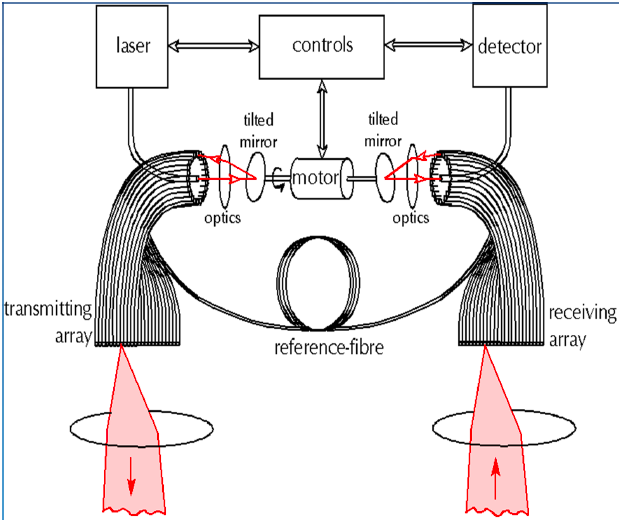
\includegraphics[height=3cm]{figure/Chapter3/光纤扫描原理}}
			\subfloat[光纤扫描脚点]{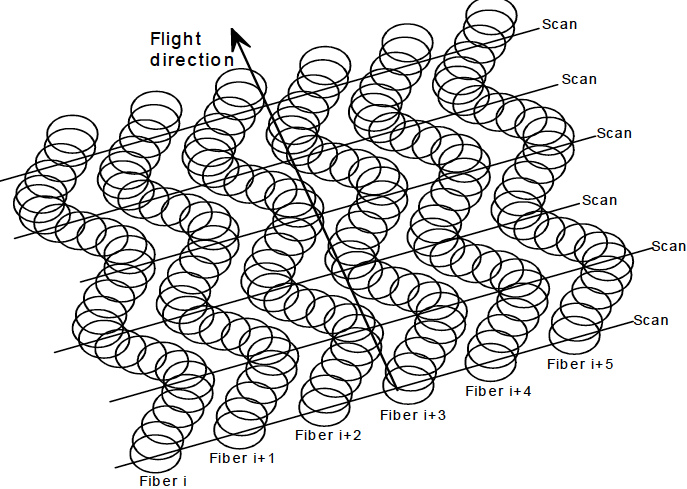
\includegraphics[height=3cm]{figure/Chapter3/光纤扫描脚点}}
			\caption{光纤扫描}
			\label{fig:光纤扫描}
		\end{figure}
\end{enumerate} % 机载LiDAR系统四种典型的扫描方式

\subsection{扫描线形状} % Subsection	扫描线形状	----------------------------------------
扫描线在地面形成的形状不仅取决于激光扫描装置及其工作方式,也取决于飞行方向、飞行速度和地形。

沿着扫描方向对地面目标的连续扫描,是一种等角度步进扫 ,激光所照射的那些点并不是等间距的。由于有时扫 速度不平衡,或加快或减慢,造成扫 线边上的点出现异样,表现出不同的特征,有时就需要从所采集的数据集合中去除这些点。

\paragraph{分类}
\begin{enumerate}
	\item \textbf{按扫描方式}:摆镜扫描;旋转棱镜扫描;椭圆扫描;光纤扫描。
	\item \textbf{按激光扫描方向}:单向扫描;双向扫描。
	\item \textbf{按扫描轨迹}:线扫描;椭圆扫描。
\end{enumerate}

\section{LiDAR数据获取处理}

\paragraph{机载LiDAR获取的数据}
\begin{itemize}
	\item 距离数据、强度信息、CCD等遥感数据
	\item DGPS系统及INS系统等定位定姿数据、航迹文件
	\item 激光点分布模式与技术数据等辅助数据
\end{itemize}
这些信息数据必须通过同步信号,保持相互关联、匹配,才能使用!

\subsection{离线时间同步方案}如图\ref{fig:离线时间同步方案}所示。
\begin{itemize}
	\item POS数据和激光扫描数据存储在不同PC机硬盘中。
	\item POS数据与GPS时间相关,激光扫描数据与PC1的计算机内部时间相关。
	\item PC1与PC2借助GPS的PPS信号关联。
\end{itemize}
\begin{figure}[htbp]
	\centering
	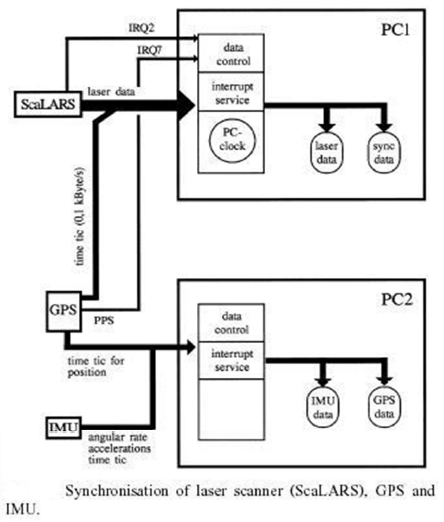
\includegraphics[width=0.5\linewidth]{figure/Chapter3/离线时间同步方案}
	\caption{离线时间同步方案}
	\label{fig:离线时间同步方案}
\end{figure}

\subsection{机载LiDAR系统对地定位方程}

\paragraph{摆镜扫描对地定位方程}通过激光对地面的扫描得到扫描仪与地面上各点的距离,由GPS接收机得到扫描仪的位置,由高精度姿态量测装置量测出扫描仪的姿态,即$ φ $、$ ω $、$ κ $角度,由这些量测值可计算出地面点的三维坐标。

设地面点$ P $在地面坐标系中的坐标为$ (X,Y,Z)_p $, $ P $在传感器坐标系中的坐标为$ (U,V,W)_P $,投影中心$ S $在地面坐标系中的坐标为$ (X_S,Y_S,Z_S) $,传感器的姿态角为$ (\varphi,\omega,\kappa) $,则通用的构象方程为
\begin{equation}
\begin{pmatrix}
X \\ Y \\ Z
\end{pmatrix}_P = \begin{pmatrix}
X_S \\ Y_S \\ Z_S
\end{pmatrix} + \symbf{A} \begin{pmatrix}
U \\ V \\ W
\end{pmatrix}_P
\end{equation}
其中,
\begin{equation}
\symbf{A} = \begin{pmatrix}
a_1 & a_2 & a_3 \\
b_1 & b_2 & b_3 \\
c_1 & c_2 & c_3 
\end{pmatrix}
\end{equation}
是传感器坐标系相对于地面坐标系的旋转矩阵,是传感器姿态角的函数。

对于每一个脉冲,有
\begin{align}
	\begin{split}
	x & = 0 \\
	y & = S \sin \theta \\
	z & = S \cos \theta
	\end{split}
\end{align}
式中,$ \theta $是扫描线方向与$ Z $轴夹角,由编码器按固定的激光脉冲间隔给出;$ S $是激光测距。

代入构像方程,有扫描线定位方程
\begin{equation}
\begin{pmatrix}
X \\ Y \\ Z
\end{pmatrix}_P = \begin{pmatrix}
X_S \\ Y_S \\ Z_S
\end{pmatrix} + \symbf{A} \begin{pmatrix}
0 \\ S\sin\theta \\ S\cos\theta
\end{pmatrix}_P
\end{equation}

\paragraph{椭圆扫描定位方程}
\begin{equation}
\begin{pmatrix}
X_P \\ Y_P \\ Z_P
\end{pmatrix} = \begin{pmatrix}
X_G \\ Y_G \\ Z_G
\end{pmatrix} + \symbf{A} \begin{pmatrix}
-S\sin 2\delta \sin \gamma \\ 
S \cos 2\delta \\ 
-S \sin 2\delta \cos \gamma
\end{pmatrix}
\end{equation}

\section{机载LiDAR数据获取新技术} %% Section	全球定位系统技术	========================================
\paragraph{数字化全波形技术}如图\ref{fig:数字化全波形技术}所示。
\begin{figure}[htbp]
	\centering
	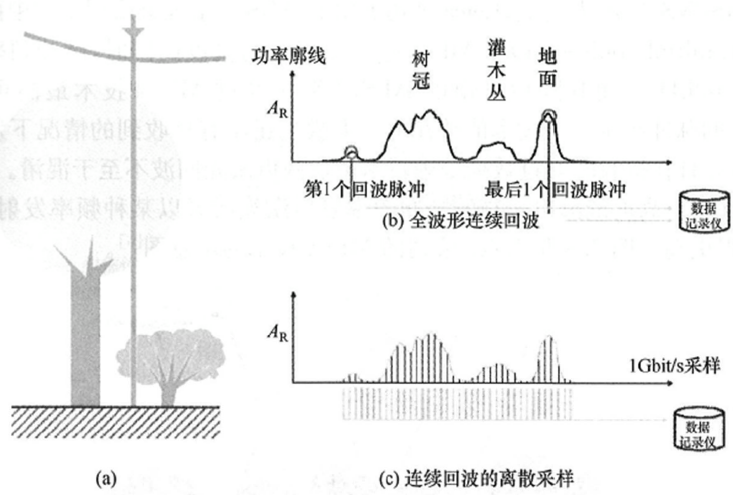
\includegraphics[width=0.7\linewidth]{figure/Chapter3/数字化全波形技术}
	\caption{数字化全波形技术}
	\label{fig:数字化全波形技术}
\end{figure}

\paragraph{空中内插多脉冲技术}如图\ref{fig:空中内插多脉冲技术}所示。
\begin{figure}[htbp]
	\centering
	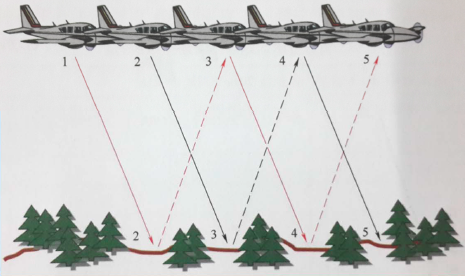
\includegraphics[width=0.7\linewidth]{figure/Chapter3/空中内插多脉冲技术}
	\caption{空中内插多脉冲技术}
	\label{fig:空中内插多脉冲技术}
\end{figure}

\paragraph{双扫描仪组合技术}如图\ref{fig:双扫描仪组合技术}所示。
增加地面激光脚点密度的方法:
\begin{itemize}
	\item 直接的方法就是增大激光脉冲的重复频率和扫描仪的扫描频率。
	\item 多脉冲技术可以通过增加激光脉冲的重复频率来达到这个目的,但是扫描仪的扫描频率由于各方面的限制很难有大幅度的提升。
	\item 双激光雷达组合的系统便应运而生。通过搭载两个激光扫描仪,并使其同时工作,可显著提高地面激光脚点密度。
\end{itemize}

\begin{figure}[htbp]
	\centering
	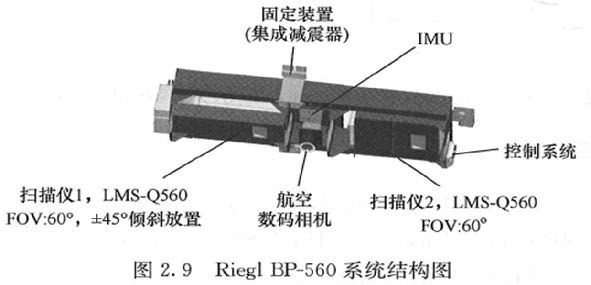
\includegraphics[width=0.7\linewidth]{figure/Chapter3/双扫描仪组合技术}
	\caption{双扫描仪组合技术}
	\label{fig:双扫描仪组合技术}
\end{figure}


\end{document}